\documentclass[a4paper, 12pt, oneside]{book}
\usepackage[utf8]{inputenc}
\usepackage[margin=3cm, bindingoffset=1cm]{geometry}
\linespread{1.5}
\usepackage[backend=biber, sorting=none]{biblatex}
\addbibresource{bib.bib}
\usepackage{float}
\usepackage{csquotes}
\usepackage{subfig}
\usepackage{graphicx}
%\usepackage{indentfirst}
\usepackage{fancyhdr}
\usepackage{xcolor}
\usepackage[acronym]{glossaries}
\usepackage{comment}
\makenoidxglossaries
\newacronym{er}{ER}{Emotion Recognition}
\newacronym{fer}{FER}{Facial Emotion Recognition}
\newacronym{ser}{SER}{Speech Emotion Recognition}
\newacronym{ml}{ML}{Machine Learning}
\newacronym{anns}{ANNs}{Artificial Neural Networks}
\newacronym{cnn}{CNNs}{Convolutional Neural Networks}
\newacronym{rnn}{RNNs}{Recurrent Neural Networks}
\newacronym{asr}{ASR}{Automatic Speech Recognition}
\newacronym{ai}{AI}{Artificial Intelligence}
\newacronym{hci}{HCI}{Human-Computer Interaction}
\newacronym{crnn}{CRNN}{Convolutional Recurrent Neural Network}

\usepackage{amsfonts}

\setlength{\parindent}{1cm}

\pagestyle{fancy}
\renewcommand{\chaptermark}[1]{\markboth{\thechapter.\ \uppercase{#1}}{}}
\fancyhf{}
\fancyhead[C]{\textbf{\leftmark}}
\fancyfoot[C]{\thepage}
\renewcommand{\headrulewidth}{1pt}
\renewcommand{\footrulewidth}{1pt}
\usepackage[Conny]{fncychap}
%\usepackage[style=ieee]{biblatex}

\title{Tesi Magistrale}
\author{Ivan Colucci}
\date{January 2020}

\newenvironment{dedication}
  {\clearpage           % we want a new page
   \thispagestyle{empty}% no header and footer
   \vspace*{\stretch{1}}% some space at the top 
   \itshape             % the text is in italics
   \raggedleft          % flush to the right margin
  }
  {\par % end the paragraph
   \vspace{\stretch{3}} % space at bottom is three times that at the top
   \clearpage           % finish off the page
  }

\graphicspath{{images/}}
  
\begin{document}
%Frontespizio
\begin{titlepage}
    \begin{center}
        \LARGE{\uppercase{Università degli Studi di Salerno}}\\
        \vspace{5mm}
        %Dipartimento
    	\uppercase{\normalsize Dipartimento di Ingegneria del informatica }\\
    \end{center}
    \begin{figure}[H]
        \centering
        
\includegraphics[width=0.25\textwidth]{logo_unisa}
    \end{figure}
    
    \begin{center}
        %Corso di Laurea
    	\normalsize{Project in Software Engineering for Artificial intelligence}\\
    	\vspace{15mm}
    	%Titolo
        {\LARGE{\bf Experimenting with Emotional Recognition Systems}}\\
    	\vspace{3mm}
    \end{center}
    
    \vspace{7mm}
    \noindent
    \begin{center}
        %Relatore
    	{\large{ Authors:\\\bf John Carlsson, 
                 Philip Le Borne, \\
                 Sarah Ternus,
                 Lukas Runt,\\
                 Cyprien Touron Decourteix,\\
                 Jana Valentina Stefan,\\
                 Simon Dannemann,\\
                 Ergi Kokoshi}}
    	\vspace{12mm}\\
    
    \url{https://github.com/John-Carlsson/SE4AI}
    	
    \end{center}
    
    \hfill
    
    %Anno Accademico
    \centering{\large \uppercase{ Anno Accademico 2022/2023 }}

\end{titlepage}
\begin{dedication}
Dedicata a coloro che\\ ci provano ogni giorno.
\end{dedication}
%Corpo della Tesi

\tableofcontents
\thispagestyle{empty}
\clearpage

\pagenumbering{Roman}\thispagestyle{empty}
\addcontentsline{toc}{chapter}{Acronyms}
\printnoidxglossary[type=\acronymtype,title=Acronyms,nonumberlist]
\newpage 
\listoffigures
\addcontentsline{toc}{chapter}{\listfigurename}
\clearpage
%\listoftables
%\addcontentsline{toc}{chapter}{\listtablename}

%\sloppy
%\hyphenpenalty=10000
%\exhyphenpenalty=10000

\newcounter{savepage}
\setcounter{savepage}{\arabic{page}}
\pagenumbering{arabic}

%\chapter{Timeplan and Work Distribution}
%\begin{table}[]
    \centering
    \begin{tabular}{c|c}
         &  \\
         & 
    \end{tabular}
    \caption{Timeplan}
    \label{tab:timeplan}
\end{table} 

\chapter{Introduction} \label{chap:introduction}
 \noindent The field of \acrfull{er} has grown in importance as \acrfull{ai} and \acrfull{ml} have gained popularity due to its potential to transform a variety of fields and applications \cite{er-appl}. With the ongoing evolution of virtual environments, such as the Metaverse, \acrshort{er} is gaining momentum as a critical component in creating a more immersive and engaging experience. By utilizing AI algorithms to analyze various physiological responses and facial expressions, \acrshort{er} technology has the potential to enhance social interactions and emotional experiences of users in virtual environments. But not only that, \acrshort{er} can offer great benefits in many other fields as well, such as marketing, healthcare, education and \acrfull{hci} \cite{er-appl,healthcare, EGGER201935}. \par
 \noindent
 As a contribution to this change, our project aims to develop a system that recognizes emotions based on both facial and speech features. Firstly, we examine what approaches have been taken so far in chapter \ref{chap:related-work}. Then, in chapter \ref{chap:project-ideas}, we define our idea and the context of our system. In chapter \ref{chap:problem-spec}, we derive the more detailed problem description as well as the resulting goals and research questions. In chapter \ref{chap:methodology}, we sum up the methodological steps to follow in order to achieve those goals. Chapter \ref{chap:Data} covers the collection of appropriate data and their preprocessing. Then, in chapter \ref{chap:Implementation}, we pursue implementing and training our models. These are then evaluated in \ref{chap:Evaluation}. Once the performance of the models is as desired, the two approaches are combined in the final application in chapter \ref{chap:final-application}. Lastly, the report is completed with a conclusion and an outlook in chapter \ref{chap:conclusion}.



\chapter{Related Work} \label{chap:related-work}
\begin{figure}[h]
\centering
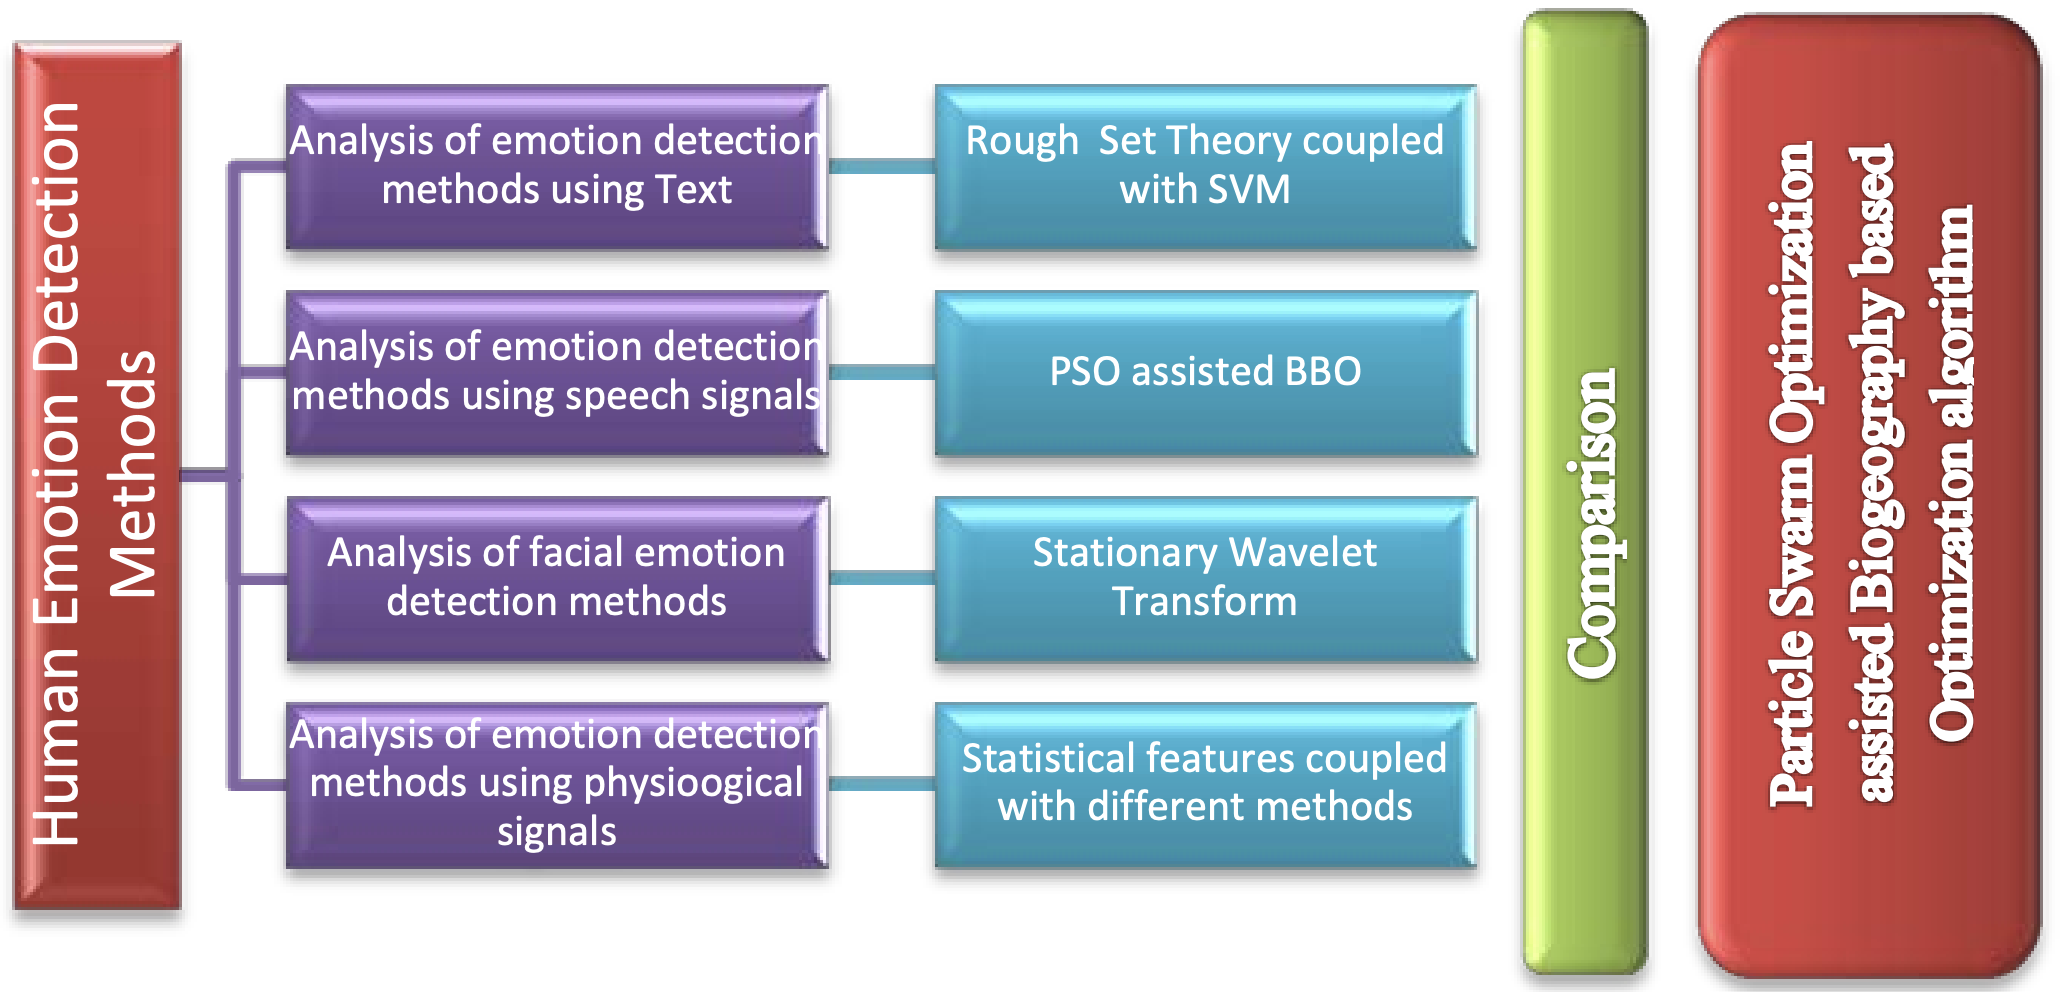
\includegraphics[width=1\textwidth]{images/Emotion-detection-survey.png}
\caption{Survey on Emotional Detection. \cite{EGGER201935}}\label{fig:survey}
\end{figure}

%\noindent The current work on emotional recognition is an active and rapidly developing field with many applications as already touched upon in chapter \ref{chap:introduction}. Like Figure \ref{fig:survey} shows, there are many possibilities to approach this. Continuing, we will focus on \acrshort{fer} and \acrshort{ser}.\\

%\noindent \acrshort{fer} is an important area of research that has many applications in \acrshort{hci} and other fields. \acrfull{cnn} have emerged as a promising approach for \acrshort{fer}, but there are numerous factors that can impact their performance. As of today, there are multiple state-of-the-art \acrshort{cnn}-based \acrshort{fer} methods that differ in their architecture, preprocessing, and training/test protocols, of which Christopher Pramerdorfer and Martin Kampel has analyzed six of in their book: Facial Expression Recognition using Convolutional Neural Networks: State of the Art\cite{pramerdorfer2016facial}.

%\noindent Especially recognizing facial expressions under naturalistic conditions is still an unsolved problem and represents a great challenge. One way to improve \acrshort{fer} performance is to overcome the bottleneck of using comparatively basic CNN architectures. A collection of modern \acrshort{cnn} has achieved a test accuracy of 75.2\% on the FER2013 dataset\cite{FER2013}. Outperforming previous works without requiring auxiliary training data or face registration \cite{pramerdorfer2016facial}.

%\noindent In the area of \acrshort{ser} the research is ongoing. Also, in the specific branch of \acrshort{hci} \acrshort{cnn} are commonly used for feature extraction and classification in \acrshort{ser}. Besides, \acrfull{rnn} (especially Gated Recurrent Unit architectures) are also effective methods for emotion recognition through speech. In this case the highest accuracy scored was 97.47\%. \cite{GRU}.

%\noindent It is also interesting to have a look at the transformer-based models, which recently were used for \acrshort{ser} with promising results \cite{transform}. \acrshort{ser} under realistic conditions presents several challenges, including the variability in speech patterns and background noise.


% NEW VERSION --

\noindent Due to the fact that the current research and development of the emotional recognition is an active and rapidly progressing field in the Human Computer Interaction sector, there are lot of related works and already successfully implemented methods. The positive effects of utilizing these advanced techniques are increasing, with society recognizing the benefits they bring to various sectors such as healthcare and the public sector. \\

\noindent The paper "Emotion Recognition from Physiological Signal Analysis: A Review" \cite{EGGER201935} provides a comprehension of over hundred of papers and a detailed analysis of the methodologies used along with the dataset for facial expression recognition, physiological signals recognition, speech signals variation and text semantics (see Figure \ref{fig:survey}). As a logical consequence we will focus on the \acrshort{fer} and \acrshort{ser} considering six elementary emotions: sadness, surprise, disgust, happiness, fear and anger. \\


\noindent First we will have a look at \acrshort{fer}. is pointing out two main categories of methods - feature based techniques and model based techniques. The highest accuracy was scored with the Stationary Wavelet Transform (see Figure \ref{fig:survey}) for FER with 97.47\%. Besides, the recognition of facial expression under naturalistic condition is still an unsolved problem and represents a great challenge. \\

\noindent Secondly, \acrshort{ser} instead is mainly divided into prosodic features, phonetic features, mathematical models and neural models. Here, underlining 99.47\% were scored with Particle Swarm Optimization assisted Biogeography based optimization algorithms (see Figure \ref{fig:survey}). Furthermore, \acrshort{ser} under realistic conditions presents several challenges, including the variability in speech patterns and background noise. \\


\chapter{Project Idea} \label{chap:project-ideas}
\noindent 
%The project idea is to use \acrshort{ml} algorithms that can recognize emotions in facial images (FER) and speech (SER). 
The goal of the project is to create a viable, working application that can differentiate between emotions using pictures or possibly a video (FER) and speech (SER) of the user.
The system will be developed using software engineering principles such as modular design, testing, and documentation to ensure reliability, scalability, and maintainability. The system will also incorporate a user feedback mechanism to enable active learning. \\


\noindent 
%As discussed in the previous chapters, there are plenty of areas in which such a solution can be used. It has then become a challenging problem that this field involves more and more scientists with different specializations \cite{HCSI201451}. Thus, the purpose of this project is to create a model that can aid individuals within their work or leisure by giving more context to virtual interactions with the addition of emotions. 
%\\
As discussed in the previous chapters, there are plenty of areas in which such a solution can be used. 
%For our project, we choose virtual education as the context but aim to keep our system as general as possible so that it can be utilized in other scenarios as well. 
%The use of ER in virtual education offers the possibility of dynamically adapting learning units to individual students based on their emotional feedback. 
Specializing the system on one area in particular would require us to gain additional expertise for that area which would extend the scope of the course. Thus, we decided to develop a generalized system that can be adapted to different use cases in the future. 
%By placing the focus on two approaches to ER instead of one, we hope to increase the overall performance of the ER system. 

\noindent In order to distribute the workload, we have decided to divide the group into two subgroups, each taking care of one of the approaches (see Figure \ref{fig:workload_division}). At the beginning, both subgroups will work individually on their approach. Then, to create the working application, the two approaches will be combined by a collaboration between the two subgroups.  
\\



\begin{table}
\begin{center}
\begin{tabular}{ |c|c| } 
 \hline
 Facial & Speech \\
 \hline
 Sarah Ternus & Cyprien Touron Decourteix \\ 
 John Carlsson & Jana Valentina Stefan \\ 
 Lukas Runt & Ergi Kokoshi \\ 
 Philip Le Borne & Simon Dannemann \\
 \hline
\end{tabular}
\caption{Division of workload.}\label{fig:workload_division}
\end{center}
\end{table}





\chapter{Problem Specification and Verification}\label{chap:problem-spec}
\noindent\textbf{Main problem:}
The main problem is to create a working application, based on modular design, to recognise human emotions through facial- and speech-expressions. \\


\noindent The problem will be addressed by answering the following research questions:
\begin{enumerate}

\item To which extent can emotions be recognised through the applied models? 

\item What modules are required for the application? 

\item What is necessary to combine different approaches?

\end{enumerate}

\noindent It is important to know to what extent the model can accurately predict outcomes to make the application as accurate as possible, however, a good-enough classification accuracy will be accepted as the project is time constrained.

\noindent The application is to incorporate many different mechanisms and  it is crucial to know what modules needs to be created for both approaches.

\noindent To achieve a working application by combining the approaches a general application will be incorporated by using modular design choices.
\\
\noindent Some demarcations to be aware of. A problem with user feedback is that it relies on the user to not be malicious. Because of this, the evaluation of the feedback mechanism will be done in a closed environment by the project group to ensure that all feedback is benign.

\noindent The \acrlong{gui} used to implement feedback will be limited and only functional since the project is limited by time.


\noindent When creating the models, known \acrshort{cnn} will be used by implementing them in Python. \\


\noindent The research questions will be verified as follows:

\begin{enumerate}

    \item The model will produce an accuracy of the classified emotions as a percentage. A satisfactory goal  for separate emotions would be 60\%, and for grouped emotions, 80\%. The percentages are set as a guess estimate, based on previous research.\cite{pramerdorfer2016facial}
    \item To create a viable and modular solution, it is necessary to identify which modules that are needed for each approach. Simply put, if a module is created it is necessary.
    \item To combine different approaches, they must be integrated together. The identifications of these steps are crucial to make the model modular for approaches other than the ones studied here. 
\end{enumerate}


\chapter{Methodological Steps} \label{chap:methodology}
% This is the chapter 4 that the teacher refers to
\begin{figure}[h]
\centering
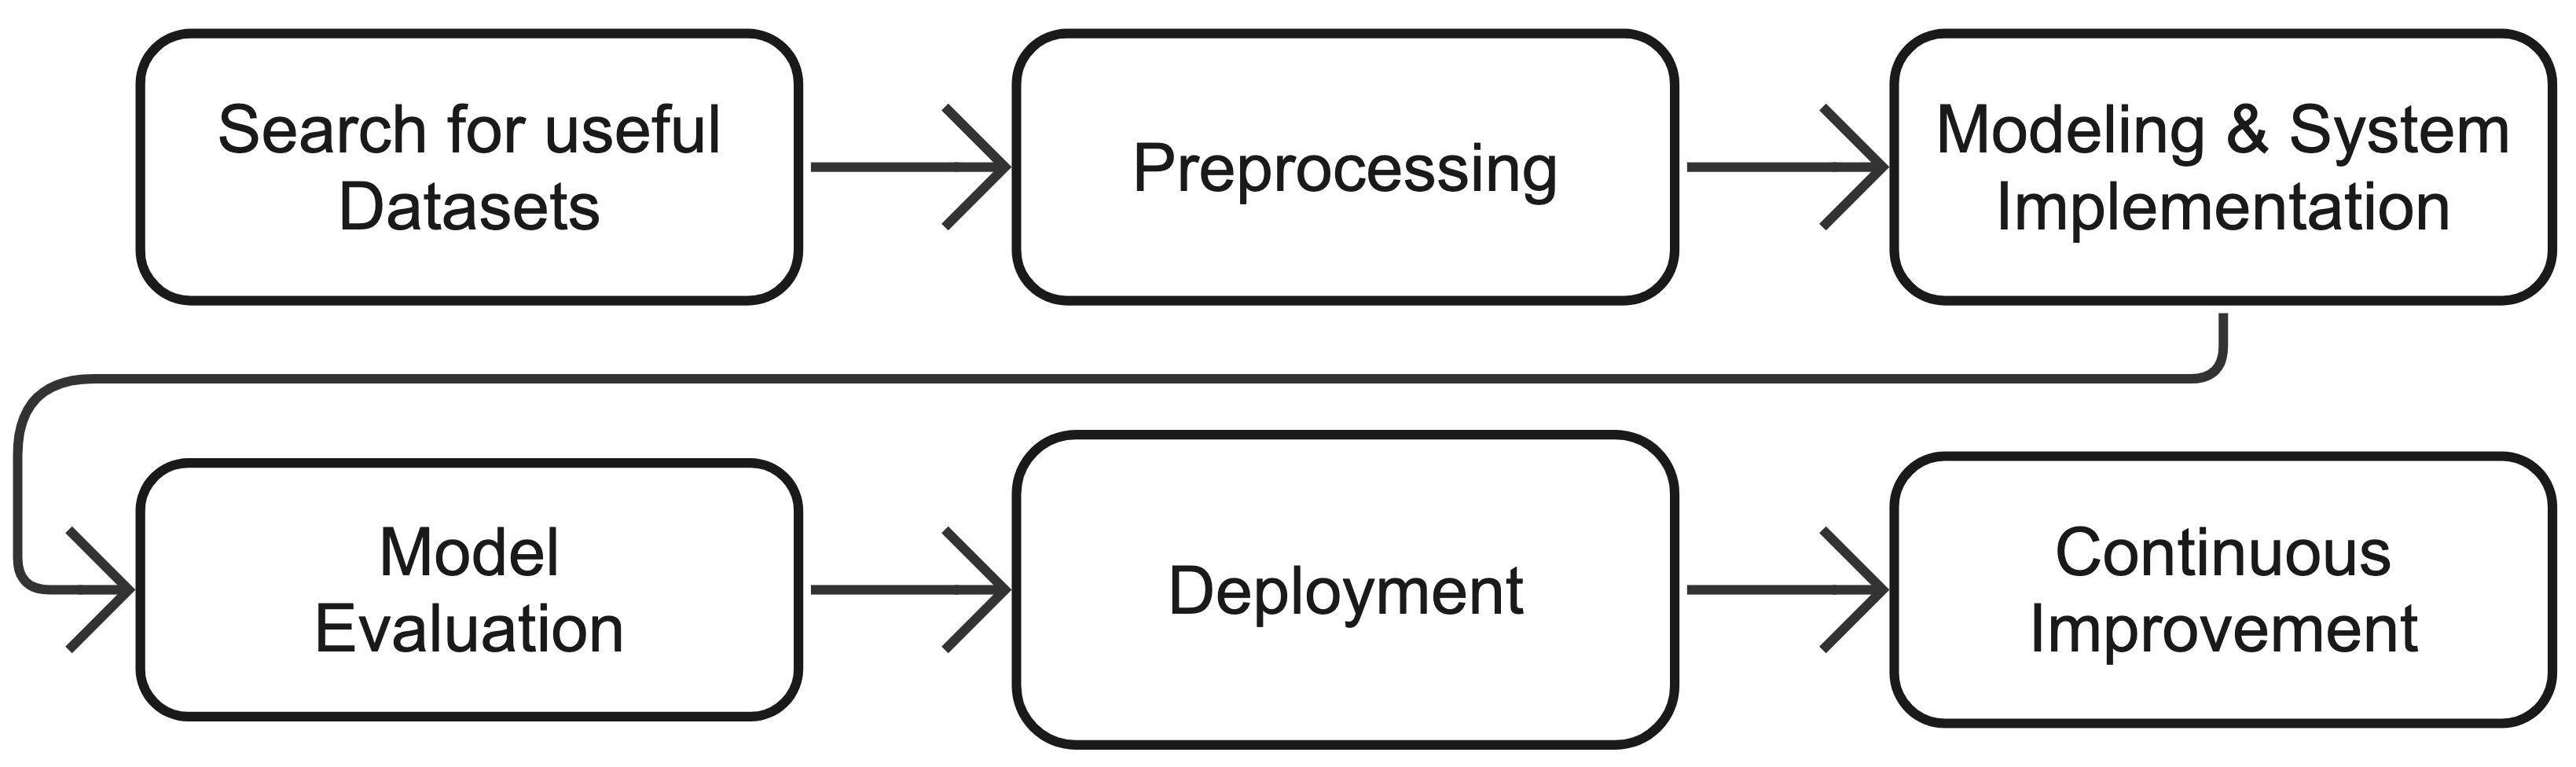
\includegraphics[width=\textwidth]{images/methodology2.png}
\caption{Methodology}\label{fig:methodology}
\end{figure}

\noindent 
%As seen in the previous section \acrshort{fer} and \acrshort{ser} is a relevant research area within various applications and fields. 
In this section, we will present the methodology for developing both a facial- and a speech emotion recognition system. Consequently, this section discusses the several methodical steps that need to be taken to address the research questions and reach the research goals.
%this section discusses several steps, for example data collection, preprocessing, modeling and model evaluation, including the user feedback. 


\begin{enumerate}
\color{blue}
    \item \textbf{Data Collection:}
    The first step in the project report is the data collection. This step is relevant, because the performance of emotion recognition models is highly dependent on the quality and diversity of the dataset used to train them. Therefore, it is necessary to collect a large and diverse dataset of both facial and speech emotional expressions to train and test the models. During the data collection process, the licence to use the corresponding data is considered.
    
    \item \textbf{Data Preprocessing:}
    Secondly comes the data preprocessing, which is crucial for cleaning and preparing the collected data for training the model. This step may involve data augmentation and feature extraction, depending on the specific techniques used for \acrshort{fer} and \acrshort{ser}. Data preprocessing is also essential for ensuring that the dataset is balanced and is a main step to ensure the model can generate good results.
    
    \item \textbf{Model and System Implementation:}
    The next crucial step is the implementation and training of the \acrshort{fer} and \acrshort{ser} models. Hereby, different machine learning frameworks may be used. Lastly, both models will be integrated into two individual pipelines that should be able to process real-time data streams and predict the according emotion of the user. 
    
    \item \textbf{Model Evaluation:}
    The model evaluation, which is the fourth phase, aids in determining how well the \acrshort{fer} and \acrshort{ser} models operate, utilizing evaluation criteria like accuracy, precision, and recall. Model evaluation is crucial for deciding which models are best suitable and for identifying any weaknesses or potential areas for improvement.
        
    \item \textbf{Deployment:}
    Thereafter, the final application will be deployed, whereby the \acrshort{fer} and \acrshort{ser} models will be integrated into a single system. Deployment is essential for testing the system's performance in real-world scenarios and verifying that the models can work together effectively and the feedback system works.
    
    \item \textbf{Continuous Improvement:}
    Lastly, the final step is a continuous improvement of the system. This involves continually updating and improving the \acrshort{fer} and \acrshort{ser} models e.g. through user feedback. This step may later also involve monitoring the system's performance, as well as adding new features and functionality to the system. Continuous improvement is essential for ensuring that the \acrshort{fer} and \acrshort{ser} models can adapt to new data and different real-world scenarios and can continue to perform well over time, which is according to our research goal. 
\end{enumerate}

\noindent By following these steps, we aim to develop a robust and accurate system that can recognize emotions from facial expressions and speech signals and can be used in various applications such as healthcare, marketing and security.



%\section{Facial Emotion Recognition}
%\begin{comment}
To Do:
\begin{itemize}
\color{red}
     \item Define the specific goals of the study, e.g., which characteristics of the problem will be used to assess the validity of the proposed solution?
     \item Design an empirical strategy to address the specific goals established.
    \item The pipeline implemented must be shown to work on a non-trivial (possibly real-world) example— a toy problem is not admitted.
    \item The pipeline implemented is experimented using a dataset with 3D images.
    \item A comprehensive analysis of multiple performance indicators.
    \item Implementation of the user feedback mechanism.
\end{itemize}

\begin{enumerate}
\color{blue}
\item \textbf{Preprocessing:} Explain the steps taken to preprocess the images, such as resizing, cropping, and normalization. Also, mention any techniques used to address issues like noise or distortion in the images.
\item \textbf{Feature Extraction:} Outline the techniques used to extract features from the images. This could include handcrafted features or deep learning approaches such as convolutional neural networks.
\item \textbf{Modeling:} Explain the algorithm used to build the model for emotional recognition in images, including any modifications made to the model architecture or hyperparameters.
\item \textbf{Evaluation:} Describe the evaluation metrics used to assess the performance of the model, such as accuracy, precision, recall, or F1-score. Also, mention the cross-validation approach used to ensure the generalization of the model.
\item \textbf{Comparison with Previous Studies:} Compare the results of your model with those of previous studies on emotional recognition in images, if any.
\item \textbf{Ethical Considerations:} Discuss the ethical considerations related to the use of image data, such as ensuring the privacy and confidentiality of the participants in the dataset.
\item \textbf{Limitations and Future Work:} Mention the limitations of your study and outline the future work that can be done to improve the emotional recognition in images.
\end{enumerate}
\end{comment}

\begin{figure}[h!]
\centering
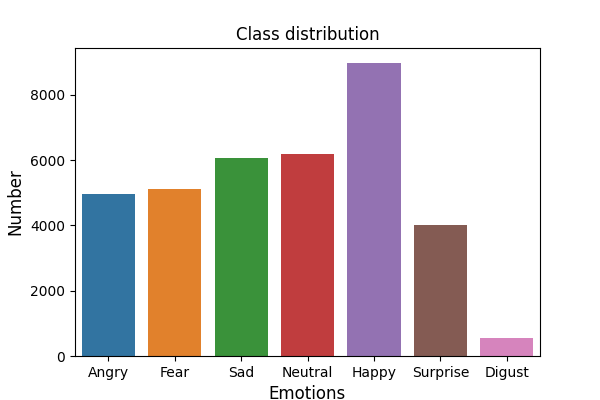
\includegraphics[scale=0.8]{barplot1.png}
\caption{Barplot of the distribution of the different classes of emotion.}\label{fig:emo-distribution}
\end{figure}

\begin{enumerate}
\item \textbf{Data Collection:} %The fer2013 dataset is handled according to the terms of the Open Database License (ODbL), which states the following: "The Licensor grants to You a worldwide, royalty-free, non-exclusive, perpetual, irrevocable copyright license to do any act that is restricted by copyright over anything within the Contents, whether in the original medium or any other. These rights explicitly include commercial use, and do not exclude any field of endeavour. These rights include, without limitation, the right to sublicense the work." \cite{odbl} We may use additional datasets provided by kaggle or other sources. 

To recognize emotions in images, the kaggle dataset \textbf{FER2013} \cite{FER2013} will be used. This dataset was prepared by Pierre-Luc Carrier and Aaron Courville as part of an ongoing research project and contains $35,887$ images, displaying the emotions anger, fear, sadness, neutralilty, happiness, surprise and disgust. Hereby, Figure \ref{fig:emo-distribution} represents the corresponding distribution of those emotions. Moreover, this dataset includes people from different genders, ethnicities and ages. Furthermore, the FER2013 dataset is handled according to the terms of the Open Database License (ODbL), which states the following: ``The Licensor grants to You a worldwide, royalty-free, non-exclusive, perpetual, irrevocable copyright license to do any act that is restricted by copyright over anything within the Contents, whether in the original medium or any other. These rights explicitly include commercial use, and do not exclude any field of endeavour [...].'' \cite{odbl} We may also use additional datasets provided by kaggle or other sources.

\begin{figure}[h]
\centering
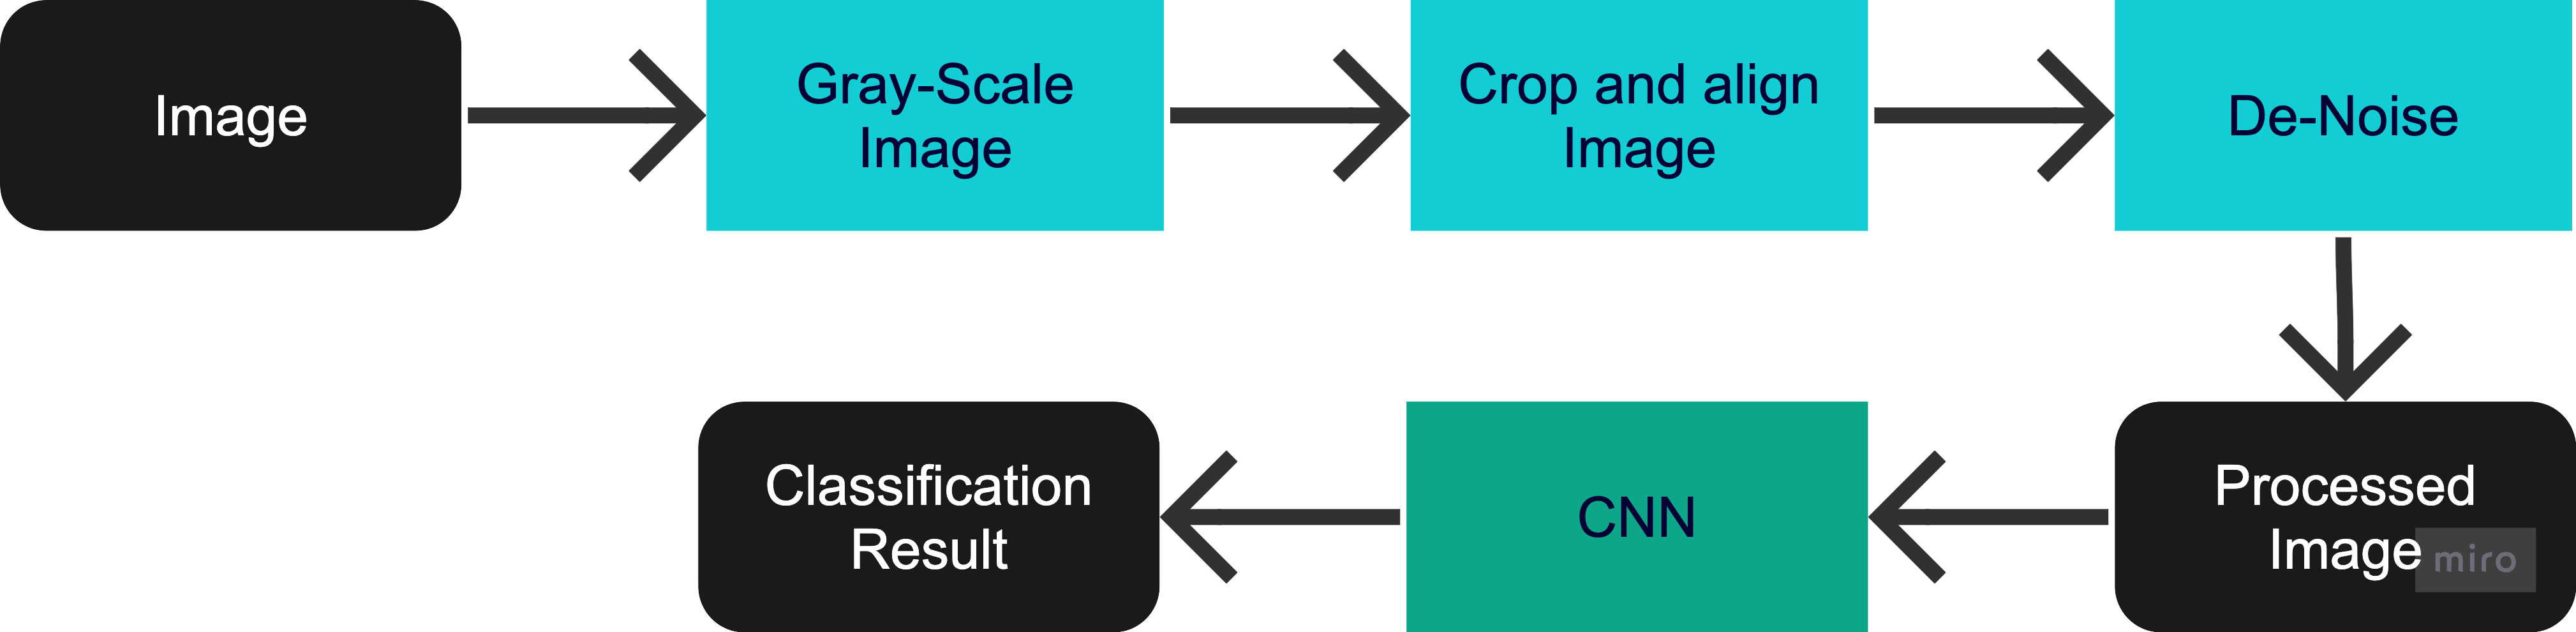
\includegraphics[width=0.9\textwidth]{images/fer-preprocessing-modelling.png}
\caption{Preprocessing and Modeling.}\label{fig:prep-mod}
\end{figure}

\item \textbf{Preprocessing:}
Before using the datasets, they will be preprocessed to exclude irrelevant images/emotions. Data preprocessing includes reducing different types of noises, resizing the picture, and aligning facial features. The method typically used to achieve the results is the eye selection method. Figure \ref{fig:emo-distribution} provides an example image of the different facial expressions with their corresponding labeled emotion. 
The \textit{FER2013} dataset provides preprocessed and labeled grayscaled images of facial emotions. We will however implement a pipeline to process new images. This will contain the following steps. The first step is to convert the (RGB) color image to a grayscale image. The colors in images can often contain clutter and hinder the model form detecting faces accurately. After the grayscale conversion, the next step is to crop and align the images, so that we are left only with the face. We should mention, that in this step we have to consider the resolution of the image and if the crop is still usable after the crop. The next step is to de-noise the image and apply filtering. De-noising the image will amplify and enhance the meaningful features of an image while reducing background noise.   Filtering is the process of altering properties of the image, for example contrast and saturation. For grayscaling and cropping the image we will use the OpenCV library.

\item \textbf{Modeling:}
Afterwards, a CNN with 2D convolutional layers will be used. This approach has been shown to be effective for image recognition tasks. We will experiment with the layers and parameters to try to achieve the best possible results. 

\begin{figure}[h]
\centering
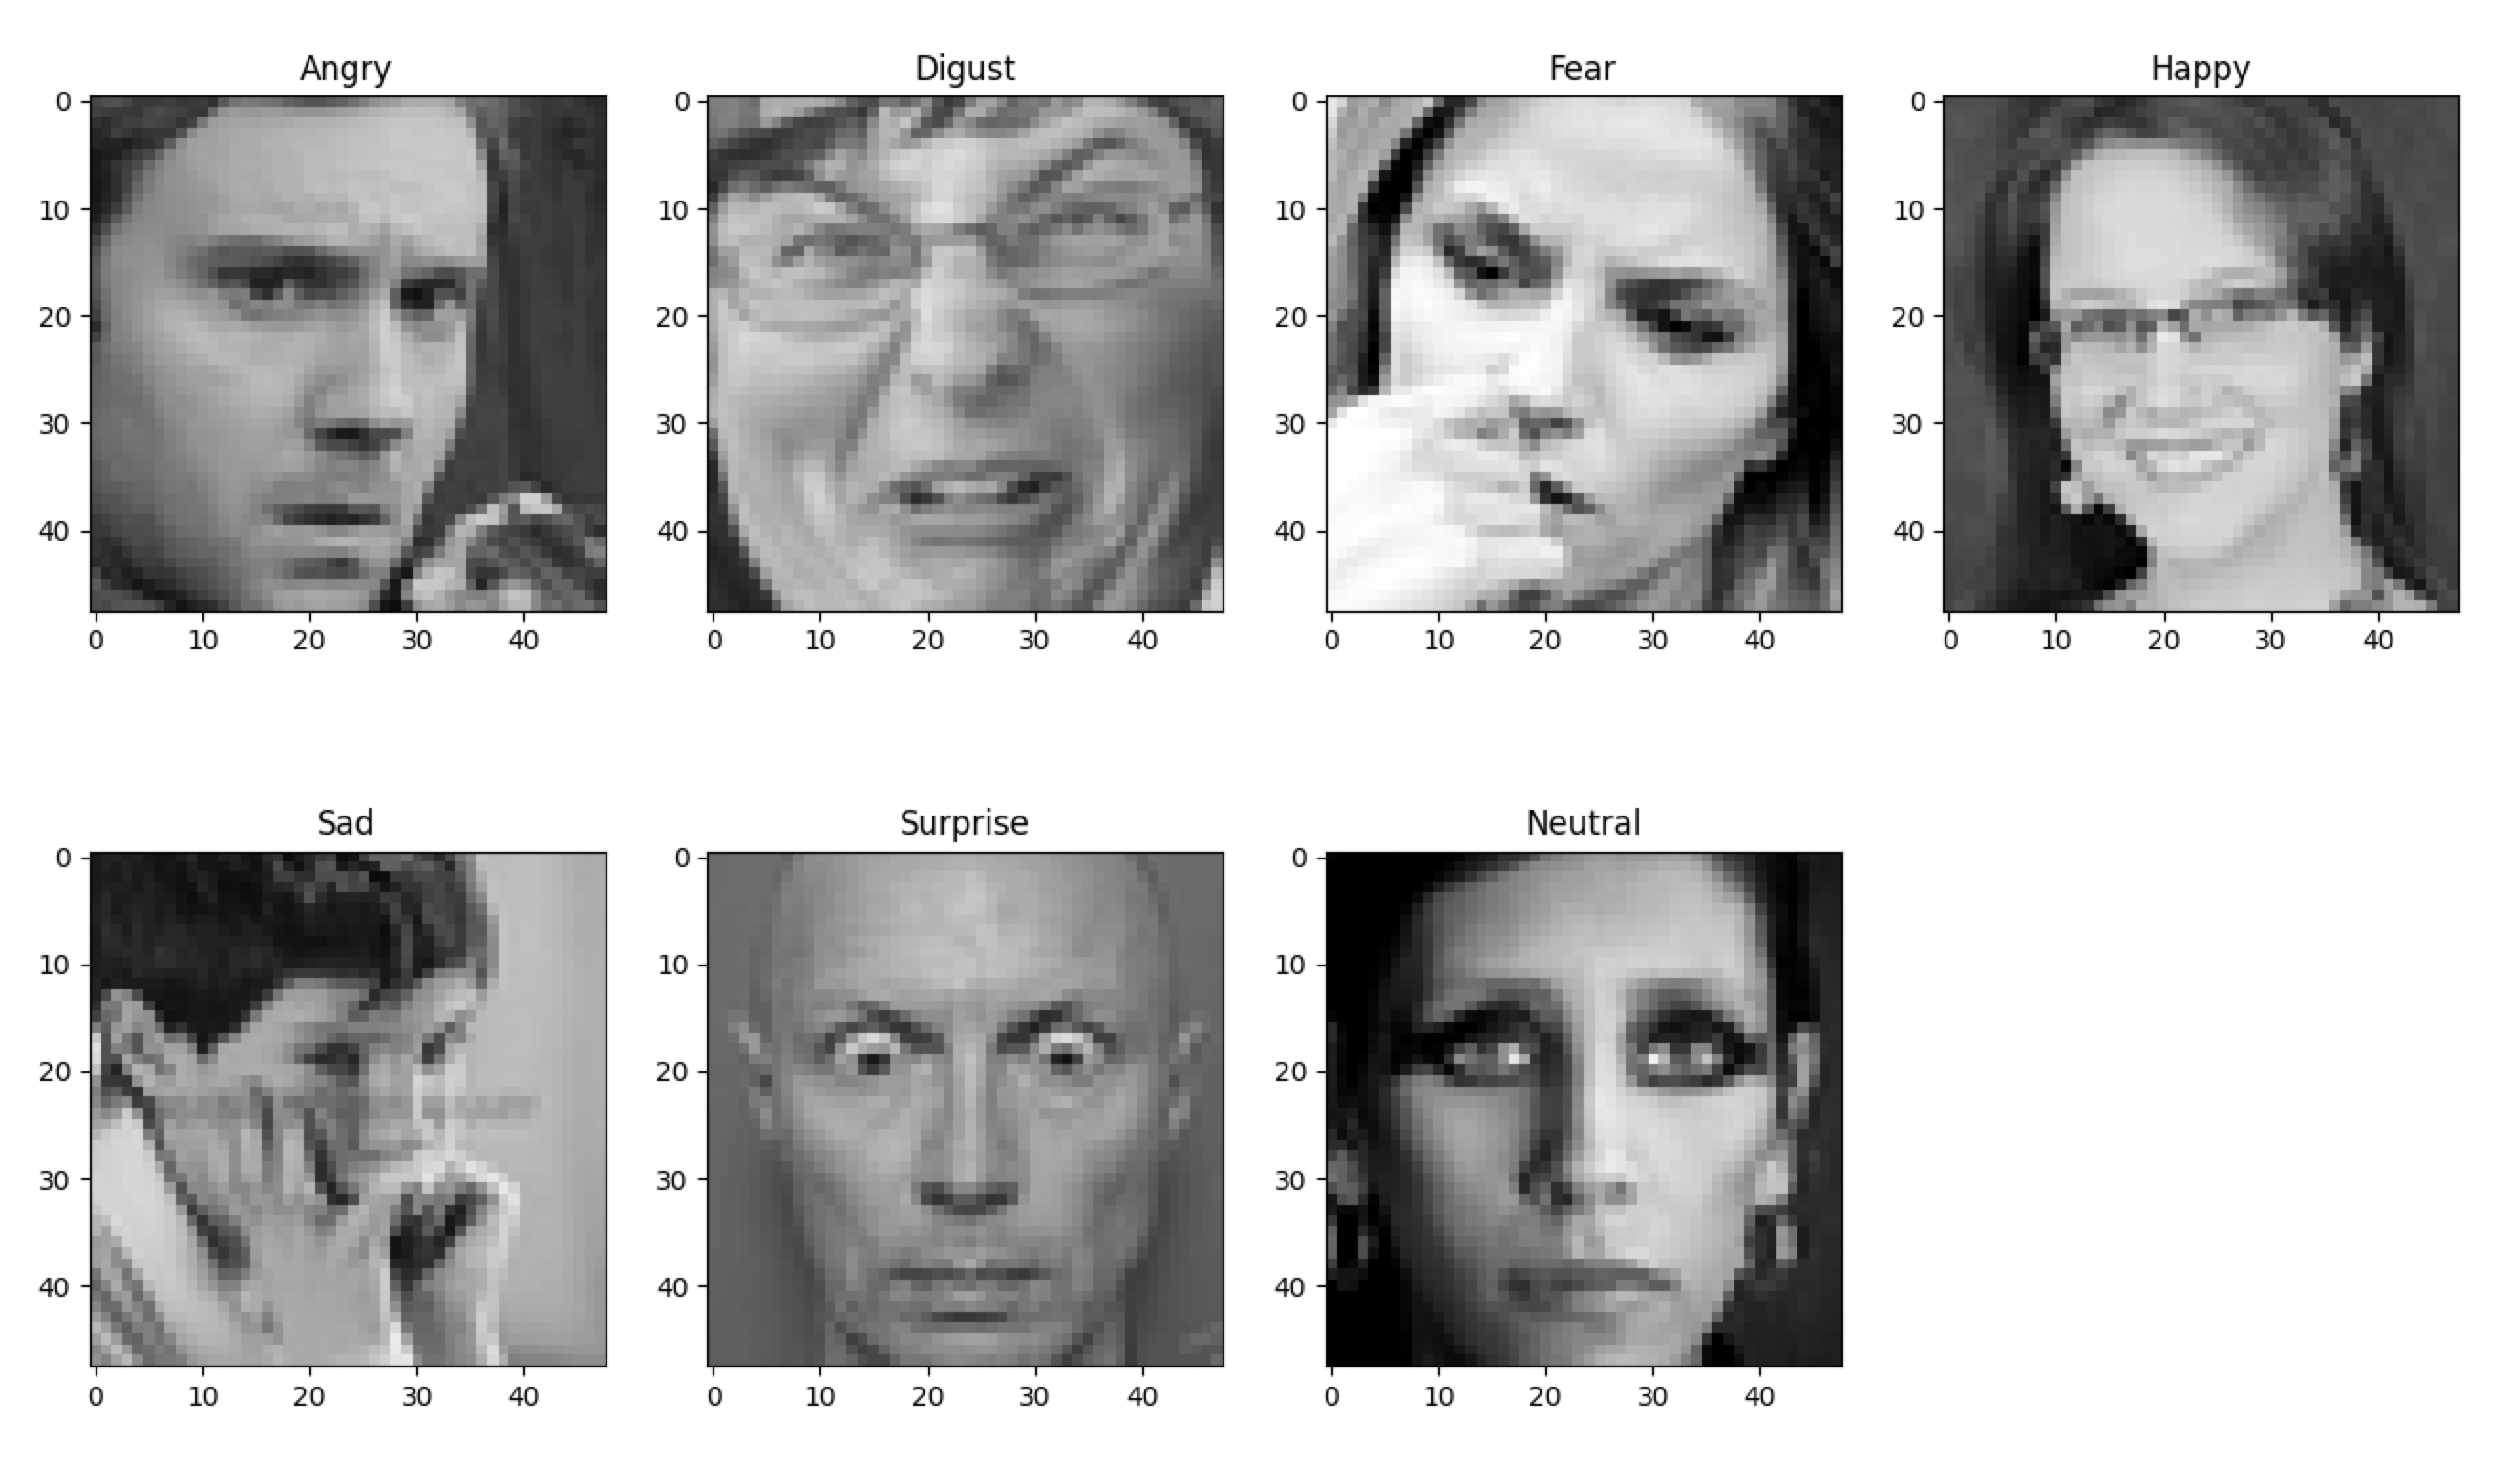
\includegraphics[width=0.9\textwidth]{faces1.png}\\
\caption{Facial expressions with corresponding emotions. \cite{FER2013}}\label{fig:faces}
\end{figure}

\newpage
\item \textbf{Model Evaluation:}
After training a model, the next goal is to test the model on new data. For this we can first use the test data and measure the accuracy, precision and recall. However for more practical applications our goal would be to implement an image preprocessing pipeline to allow us to apply the trained model on real-world captured images. This can then in turn be applied to frames of a video evaluating the emotions of one person (possibly multiple people if feasible). This will also preform as an alternative to the classic metrics for quality assurance, by allowing the person captured on the image to input their actual emotion and comparing their actual emotion to the predicted one. If we collect the new labeled images that were imputed by a user, we can retrain the model with more data, if the accuracy drops below a predetermined threshold.

\begin{figure}[h]
\centering
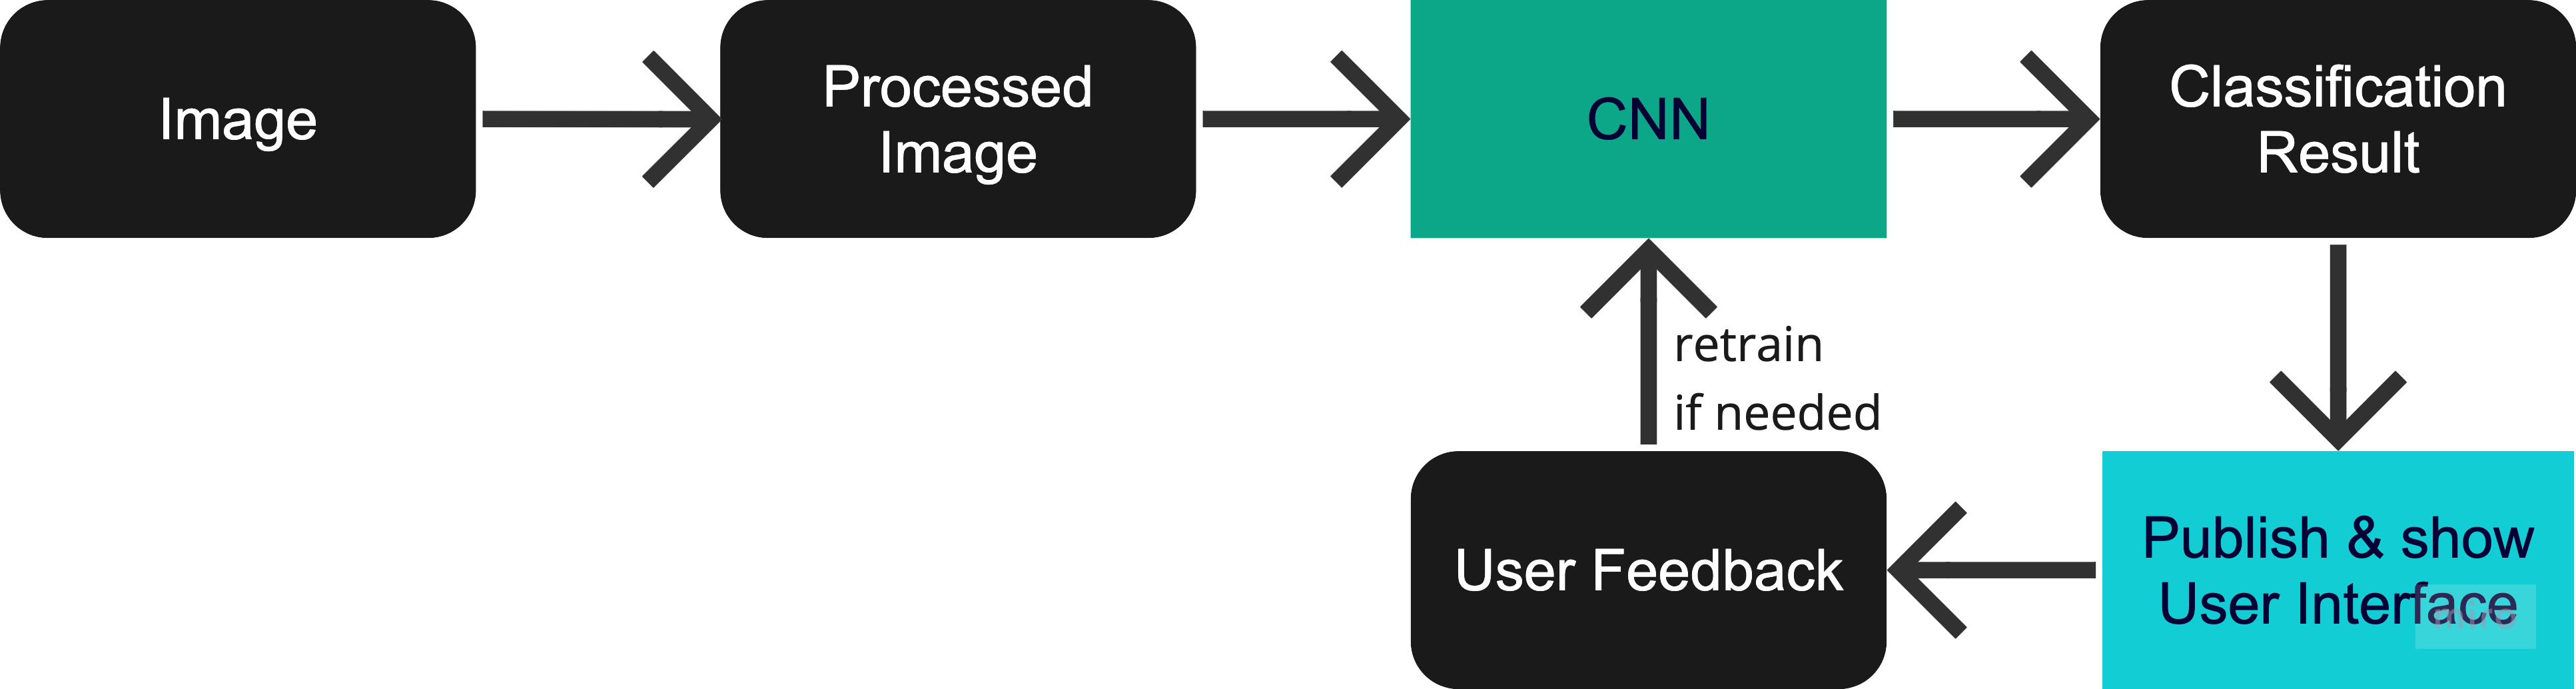
\includegraphics[width=0.9\textwidth]{images/fer-user-feedback.png}\\
\caption{General overview of the \acrshort{fer} system and user feedback}\label{fig:userfb}
\end{figure}

\end{enumerate}
\newpage

\begin{comment}
    \noindent We will implement the following files, containing classes for different models, data processing and tests: 
    \begin{enumerate}
        \item main.py
        \item ann\_model.py
        \item dataprocessing.py
        \item tests.py
    \end{enumerate}
    
    To address:
    \begin{itemize}
    \color{blue}
        \item Basic interface to better define the use case of the trained model. 
        \item Model Training: Train a deep neural network model using the preprocessed dataset.
        \item Model Evaluation: Evaluate the trained model using various metrics such as accuracy, precision, and recall.
        \item Get an Accuracy of around 65\% 
        \item System Development: Develop the emotional recognition system using the trained model and
        software engineering principles such as modular design, testing, and documentation.
        \item System Evaluation: Evaluate the developed system using various metrics such as performance, scalability, and maintainability.
        \item User Feedback: Incorporate user feedback mechanisms to improve the system’s accuracy and adaptability to new scenarios.
        \item Continuous datastreams (i.e. Video)
        \item Visualisation (Graphs, Barplots, ...) 
    \end{itemize}
\end{comment}

%\section{Preliminary results and findings}
%\section{Implications of the results}
%\section{Speech Emotion Recognition}
%\begin{enumerate}
\item \textbf{Data Collection:} \\
% Jana's task:
To train the model, we decided to use the crowd sourced CREMA-D data \cite{cremad} set that is downloadable from kaggle.com under the Open Data Commons Attribution License (ODC-By). This license allows to copy, distribute and use the database, furthermore to produce works from the database and to modify, transform and build upon it \cite{odc-by}.

The data set consists of 7,442 audio clips with the following characteristics: 
\begin{itemize}
    \item 12 different sentences
    \item six different emotions: Anger, Disgust, Fear, Happy, Neutral, Sad
    \item four different emotion levels: Low, Medium, High, Unspecified
    \item number of actors: 91
    \begin{itemize}
        \item age: ranging from 20 to 74 years
        \item ethnicity: African American, Asian, Caucasian, Hispanic, Unspecified
    \end{itemize}
\end{itemize}



\item \textbf{Preprocessing for Training:} \\
% Jana's task:
To increase the number and variety of data samples and to ensure robustness of the system to non-trivial scenarios, we will perform data augmentation in the form of random pitch shifts and time stretch transformations. Here, the python libraries Audiomentations and Librosa are useful. Both libraries are open-source and available for free. 

Then, we will calculate spectrograms from the raw audio samples by running a Fast Fourier Transform (FFT) algorithm. Here, again Librosa comes in handy. The spectrograms can then be fed into the neural networks.  

\begin{figure}[h]
\centering

\includegraphics[width=0.9\textwidth]{images/ser-preprocessing.png}\\
\caption{Preprocessing for Training.}\label{fig:ser_preprocessing}
\end{figure}

%\item \textbf{Feature Extraction:} 
\item \textbf{Modeling:} As already presented in chapter \ref{chap:project-ideas}, we are goint to use two different approaches for \acrshort{ser}, as is displayed in figure \ref{fig:ser_modeling}.\\
% Jana's task:
\emph{1. Approach: phonological information}

For the first approach, we will create a \acrfull{crnn},  i.e. a sequential neural network with 1D convolutional layers. It will take the spectrograms as input and outputs the most likely emotion associated with the input. Here, the python library Keras can be used to easily build a neural network by adding desired layers to the model. Keras is open-source and available for free. 

\emph{2. Approach: semantic information}

For the second approach, a combination of two neural networks will be used. First, an \acrfull{asr} model transforms the spectrograms into a textual representation of the utterance. This can again be done with Keras as it additionally offers APIs to pre-trained ASR models like DeepSpeech, an open-source model by Mozilla.
Then, the obtained text is assigned to an emotion by a transformer-based neural network. Here, the python library Hugging Face can be used. It is free, open-source and offers pre-trained transformer models like BERT. 
Since the ASR model and the transformer model are already pre-trained on a large corpus of data and our application scenario is kept general instead of domain-specific, it is not strictly necessary to find additional datasets for training the ASR model and the transformer model ourselves. \\

\begin{figure}[h!]
\centering
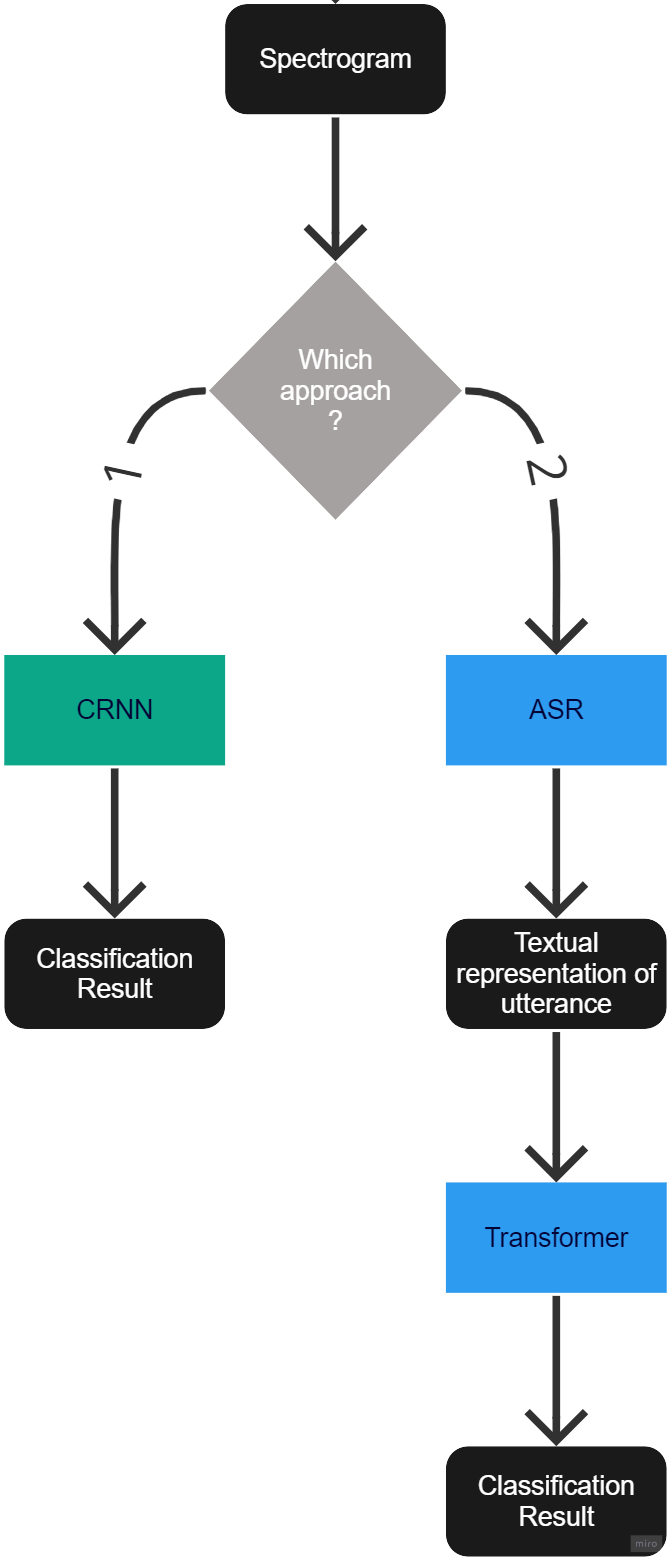
\includegraphics[scale=0.5]{images/SER_Modeling.png}\\
\caption{Modeling.}\label{fig:ser_modeling}
\end{figure}



\item \textbf{Model Evaluation:} \\
Test where we will run the model with a given input and compare its output with an expected output. The goal is to keep a track of the precision and loss of the model in training. The model must have a loss under a certain value and a precision above a certain value. During the development, we will also take advantage to unitary test for code coverage, these unitary tests will be needed to validate commit on the source control (GitHub in our case) of the project. Using this test will allow us to have an automated test pipeline that would be use for CI/CD. 

%Data splitting for Cross-Validation
%True positive (TP), True negatice (TN), False positive (FP), False negative (FN) when the model is not able to recognize any emotion.
%\begin{itemize}
%    \item Accuracy test,
%    By calculating how accurate is the model, using the following formula, $Accuracy = \frac{TP + TN}{N_{outputs}}$, we can test the success rate of the model.
%
%    \item Precision Test
%    Using the following formula, $Precision = \frac{TP}{TP + FP}$, we can test among the positive answers, the true positive rate.
%    
%    \item Sensitivity Test
%    $Sensitivity = \frac{TP}{TP + FN}$
%
%    \item Specificity Test
%    $Sensitivity = \frac{TN}{TN + FP}$
%    
%\end{itemize}

\color{black}
\item \textbf{System Development:} \\
% Jana's task
To test the speech emotion recognition in real-world scenarios, the trained neural networks will be embedded in a pipeline. 
The first step will be to record the users' utterances with a microphone. The continuous audio stream should then be cut every $x$ seconds to obtain the data samples. These will be preprocessed and fed into the neural networks. The results from both of the approaches will then be continuously published on the user interface. Here, the users indicate whether one or both of the classifications are correct and if not, what their actual emotion was. The user feedback will be stored along the respective audio sample and then used to retrain the models after the session. 
\color{blue}
%\item \textbf{System Evaluation:} including Comparison with Previous Studies: \\
% Ergi's task:
%The use of speech audio data in various applications has raised ethical considerations, particularly regarding the privacy and confidentiality of the participants in the dataset. Collecting audio data without the consent of the participants or disclosing the identity of the speakers can be a violation of privacy. Moreover, the use of audio data for purposes other than those that were originally intended can also result in ethical dilemmas. It is essential to ensure that the audio data collected is used only for legitimate purposes and that participants' personal information is kept confidential.
%\item \textbf{Limitations and Future Work:} \\
\end{enumerate}

%\section{Preliminary results and findings}
%\section{Implications of the results}

\chapter{Data Collection and Preprocessing}\label{chap:Data}
\section{\acrlong{fer}}
\subsection{Data Collection}
To recognize emotions in images, the kaggle dataset \textbf{FER2013} \cite{FER2013} will be used. This dataset was prepared by Pierre-Luc Carrier and Aaron Courville as part of an ongoing research project and contains $35,887$ images, displaying the emotions anger, fear, sadness, neutralilty, happiness, surprise and disgust. Hereby, Figure \ref{fig:emo-distribution} represents the corresponding distribution of those emotions. Moreover, this dataset includes people from different genders, ethnicities and ages. Furthermore, the FER2013 dataset is handled according to the terms of the Open Database License (ODbL), which states the following: ``The Licensor grants to You a worldwide, royalty-free, non-exclusive, perpetual, irrevocable copyright license to do any act that is restricted by copyright over anything within the Contents, whether in the original medium or any other. These rights explicitly include commercial use, and do not exclude any field of endeavour [...].'' \cite{odbl} We may also use additional datasets provided by kaggle or other sources.

\begin{figure}[h!]
\centering
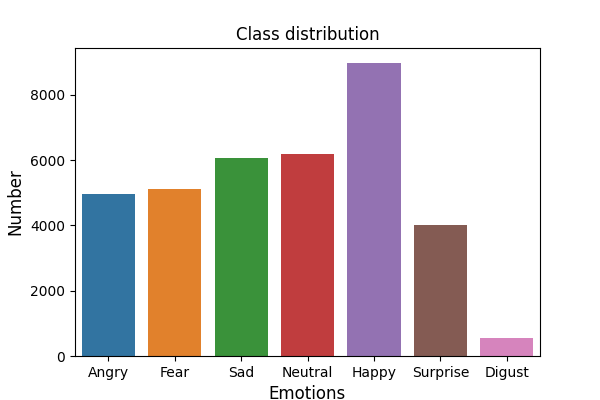
\includegraphics[scale=0.8]{barplot1.png}
\caption{Barplot of the distribution of the different classes of emotion.}\label{fig:emo-distribution}
\end{figure}

\subsection{Data Preprocessing}
Before using the datasets, they will be preprocessed to exclude irrelevant images/emotions. Data preprocessing includes reducing different types of noises, resizing the picture, and aligning facial features. The method typically used to achieve the results is the eye selection method. Figure \ref{fig:emo-distribution} provides an example image of the different facial expressions with their corresponding labeled emotion. 
The \textit{FER2013} dataset provides preprocessed and labeled grayscaled images of facial emotions. We will however implement a pipeline to process new images. This will contain the following steps. The first step is to convert the (RGB) color image to a grayscale image. The colors in images can often contain clutter and hinder the model form detecting faces accurately. After the grayscale conversion, the next step is to crop and align the images, so that we are left only with the face. We should mention, that in this step we have to consider the resolution of the image and if the crop is still usable after the crop. The next step is to de-noise the image and apply filtering. De-noising the image will amplify and enhance the meaningful features of an image while reducing background noise.   Filtering is the process of altering properties of the image, for example contrast and saturation. For grayscaling and cropping the image we will use the OpenCV library.

\begin{figure}[h]
\centering
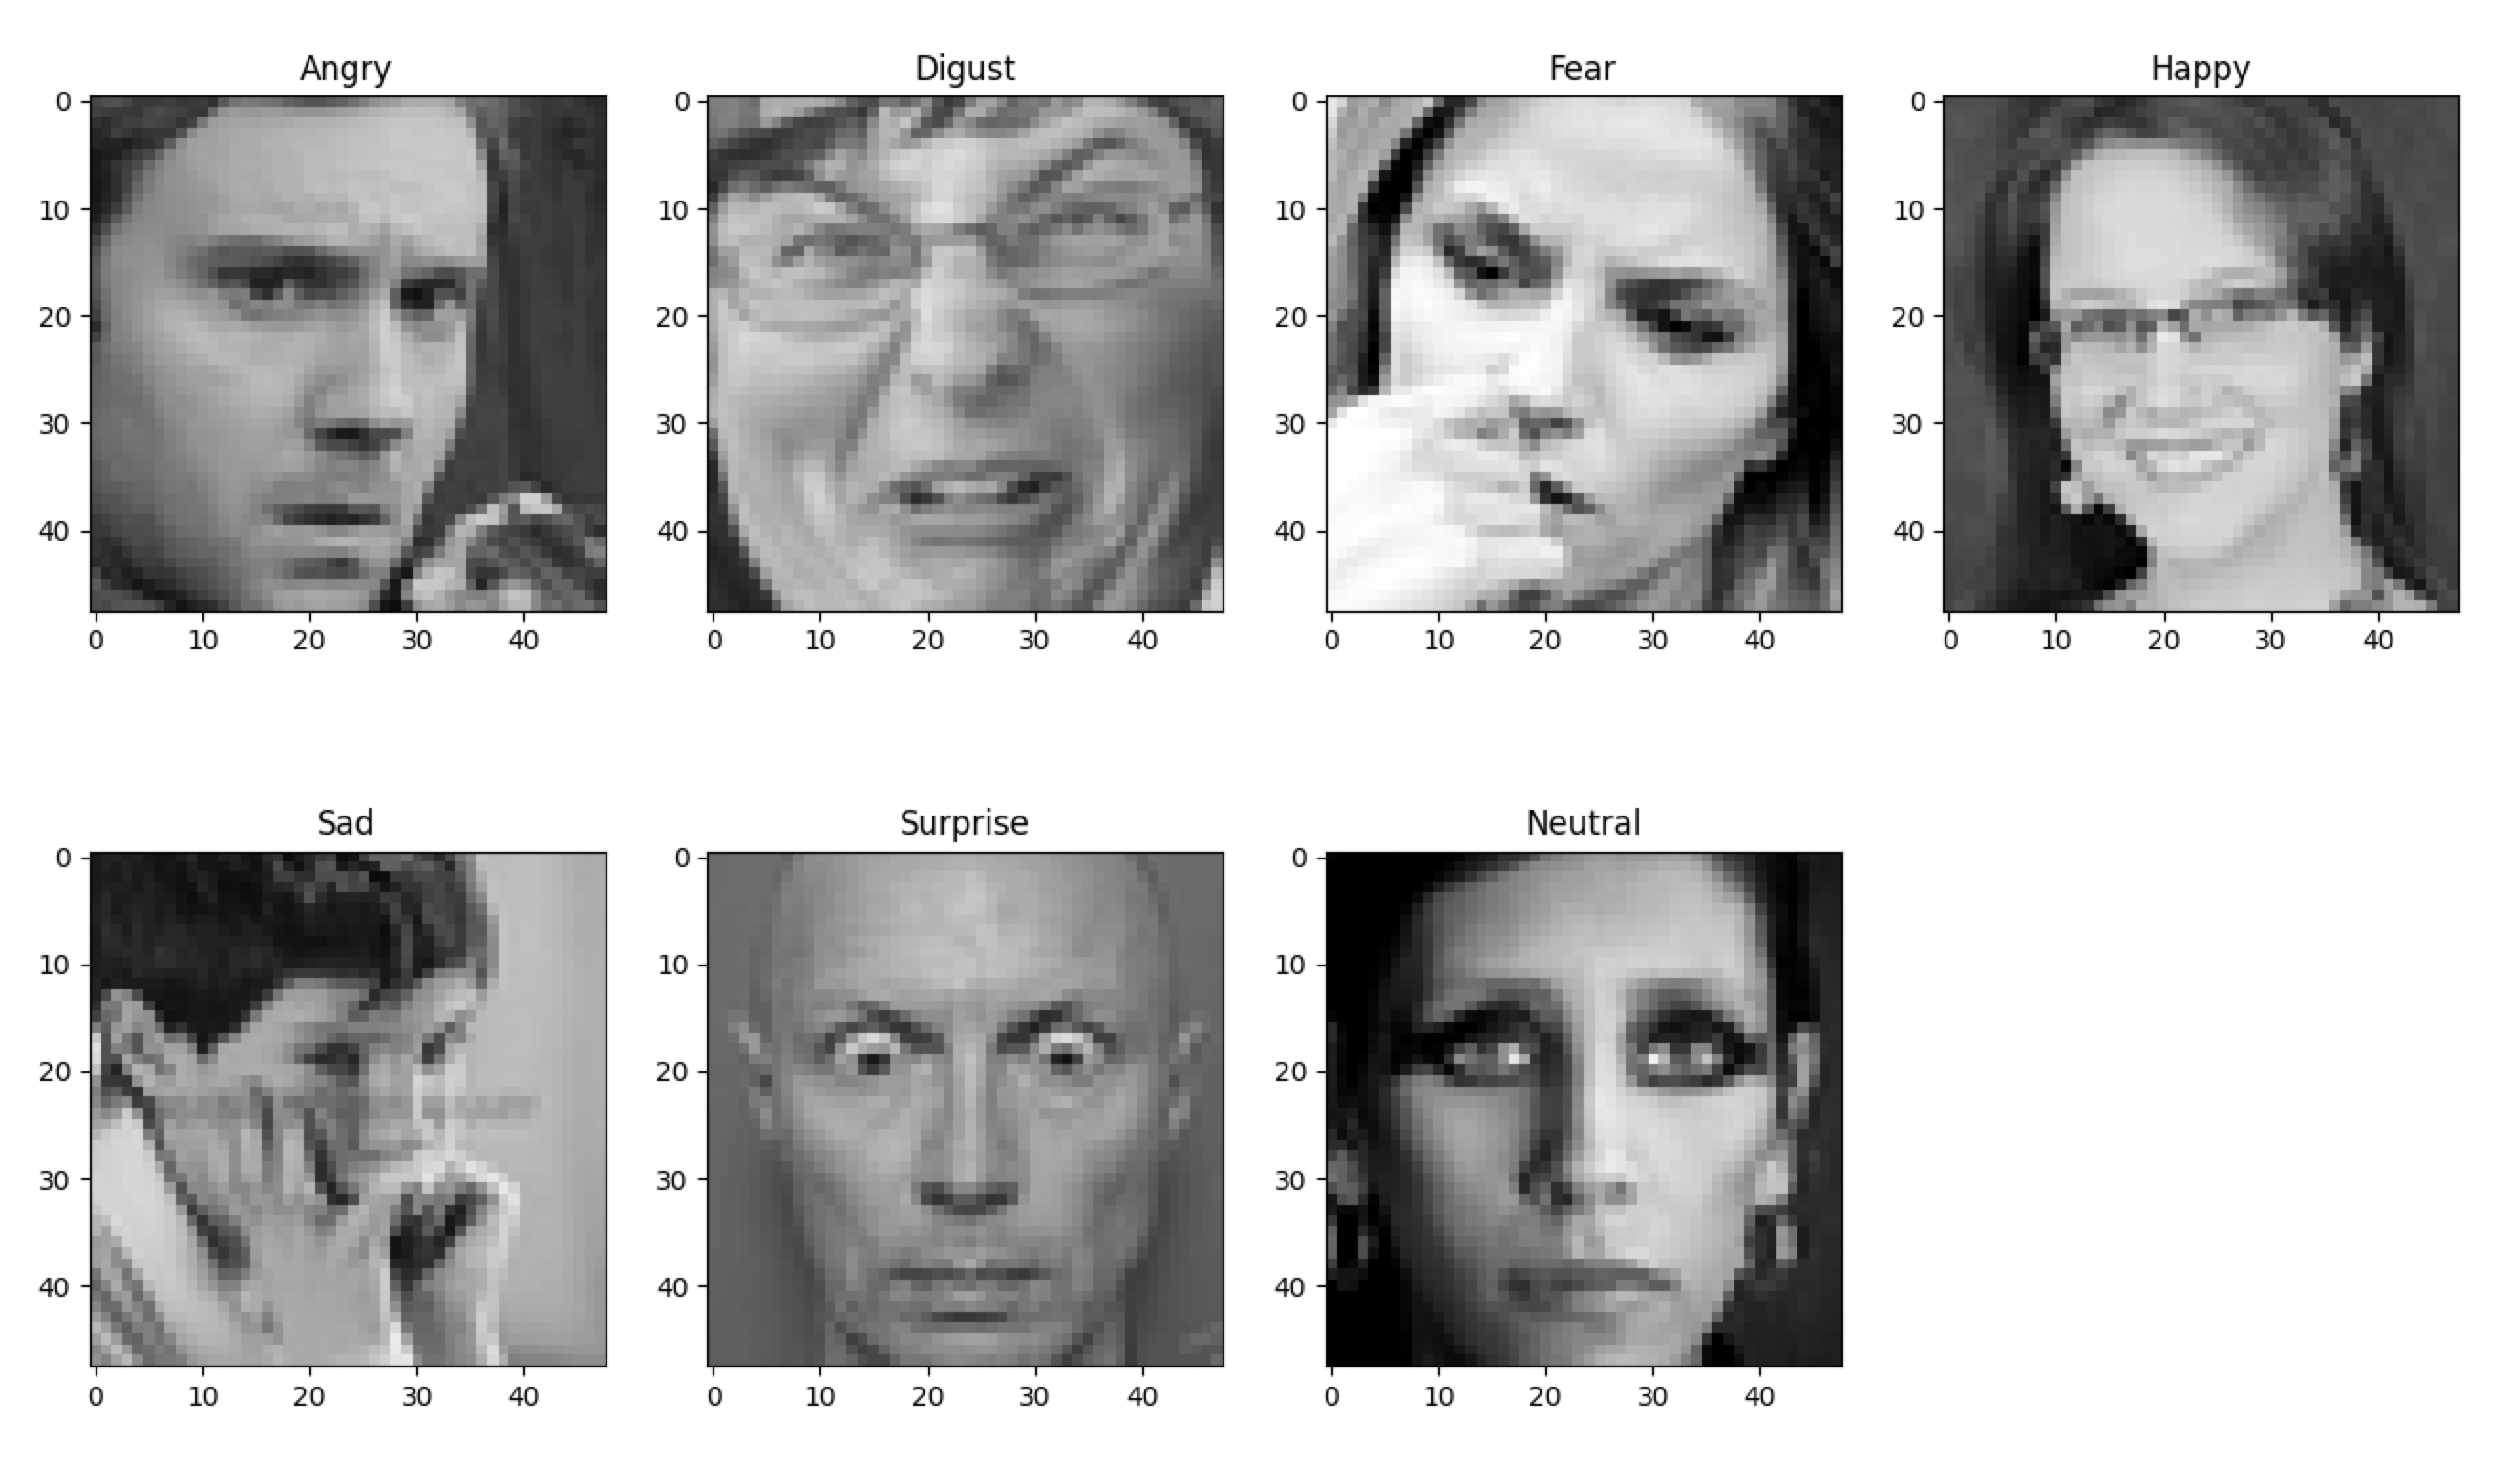
\includegraphics[width=0.9\textwidth]{faces1.png}\\
\caption{Facial expressions with corresponding emotions. \cite{FER2013}}\label{fig:faces}
\end{figure}

\section{\acrlong{ser}}
\subsection{Data Collection}
% Jana's task:
To train the model, we decided to use the crowd sourced CREMA-D data \cite{cremad} set that is downloadable from kaggle.com under the Open Data Commons Attribution License (ODC-By). This license allows to copy, distribute and use the database, furthermore to produce works from the database and to modify, transform and build upon it \cite{odc-by}. The data set consists of 7,442 audio clips with the following characteristics: 
\begin{itemize}
    \item 12 different sentences
    \item six different emotions: Anger, Disgust, Fear, Happy, Neutral, Sad
    \item four different emotion levels: Low, Medium, High, Unspecified
    \item number of actors: 91
    \begin{itemize}
        \item age: ranging from 20 to 74 years
        \item ethnicity: African American, Asian, Caucasian, Hispanic, Unspecified
    \end{itemize}
\end{itemize}



\subsection{Data Preprocessing}
% Jana's task:
To increase the number and variety of data samples and to ensure robustness of the system to non-trivial scenarios, we will perform data augmentation in the form of random pitch shifts and time stretch transformations. Here, the python libraries Audiomentations and Librosa are useful. Both libraries are open-source and available for free. 

Then, we will calculate spectrograms from the raw audio samples by running a Fast Fourier Transform (FFT) algorithm. Here, again Librosa comes in handy. The spectrograms can then be fed into the neural networks.  \\

\begin{figure}[h]
\centering

\includegraphics[width=0.9\textwidth]{images/ser-preprocessing.png}\\
\caption{Preprocessing for Training.}\label{fig:ser_preprocessing}
\end{figure}

\chapter{Model Implementation and Training}\label{chap:Implementation}
\section{\acrlong{fer}}
As the model for FER, a CNN with 2D convolution layers will be used. This approach has been shown to be effective for image recognition tasks. 
The 2D convolution layers are simple mathematical calculations in which a kernal is iteratively projected onto parts of a two dimensional matrix.
The convolution layers are used to reduce the image to its most important attributes. More specifically the convolution layers begin at detecting  similar patters and more complex ones as we increase the number of convolution layers. Though for a different example, this is visualized in Figure \ref{fig:con2dart}. Through this, important features in our example images in FER2013, for example the outline of cheeks, lips, mouth, etc. can be localized before being classified in the dense layers. This reduces the computational load in the dense layers, which in turn will provide a higher accuracy. However reducing the images to much may result in the opposite effect. 

At first it is unknown what the ideal choice of a kernal is. The values of the kernal matrix are approximated using the keras library, these are so-called trainable parameters. By either increasing or decreasing the kernal-size, we can tune the number of trainable weights of or model. 

\begin{figure}[h]
\centering
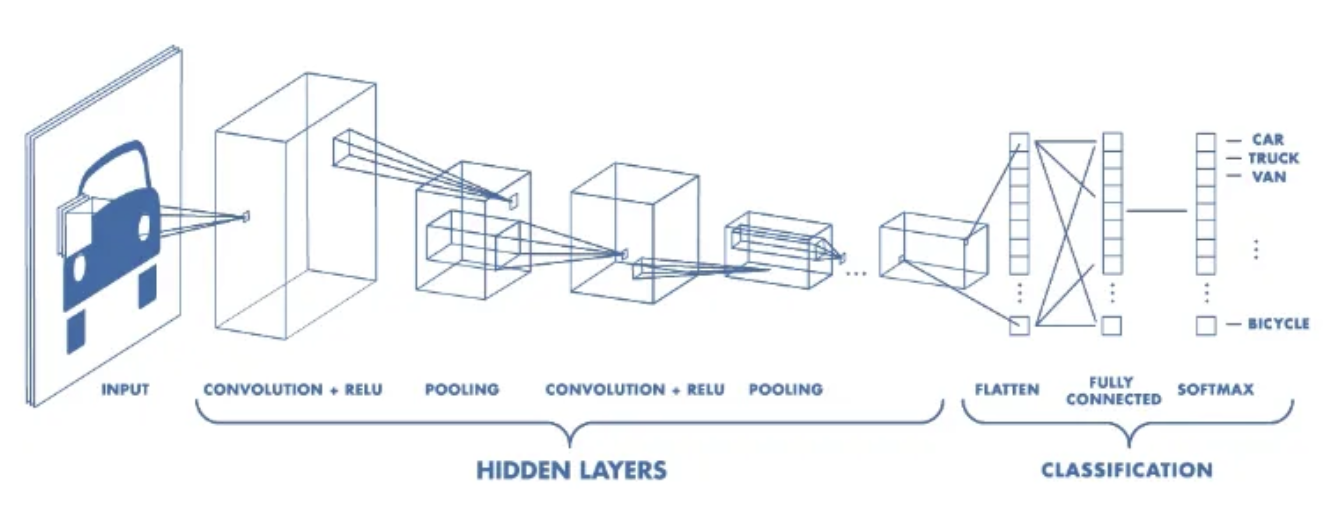
\includegraphics[width=0.9\textwidth]{images/conv2d2.png}
\caption{Structure of a 2D CNN. \cite{con2dart}}\label{fig:con2dart}
\end{figure}
In our first model we will implement six 2D Convolution Layers and three dense layers. With this we can expect an accuracy of $64\%$, however we aim to experiment with \acrshort{cnn} with a different amount of hidden layers and activation functions. In the convolution layers we have to set the following attributes: 
\begin{enumerate}
    \item Number of filters - This is the number of kernal, i.e. filters that a convolution layer will learn from. It is common that a convolution layer or network will learn many filters in parallel. This enables the network to recognize a greater amount of patterns in an image and is often refereed to as ``Computer vision''.
    \item Kernel size - The kernel is the neural network filter that moves across the image, scanning each pixel and converting the data into a smaller, or sometimes larger, format. It's good to use the kernel odd-sized kernel because of symmetry. We are interpolating the central pixel.
    \item Padding - Padding refers to the number of pixels added to an image when it is being processed by the kernel of a \acrshort{cnn}. Adding padding to an image processed by a \acrshort{cnn} allows for a more accurate analysis of images.
\end{enumerate}
We will implement a model with a similar structure as the model depicted in Figure \ref{fig:con2dart} and experiment with different parameters to try to achieve the best possible results. 

\begin{figure}[h]
\centering
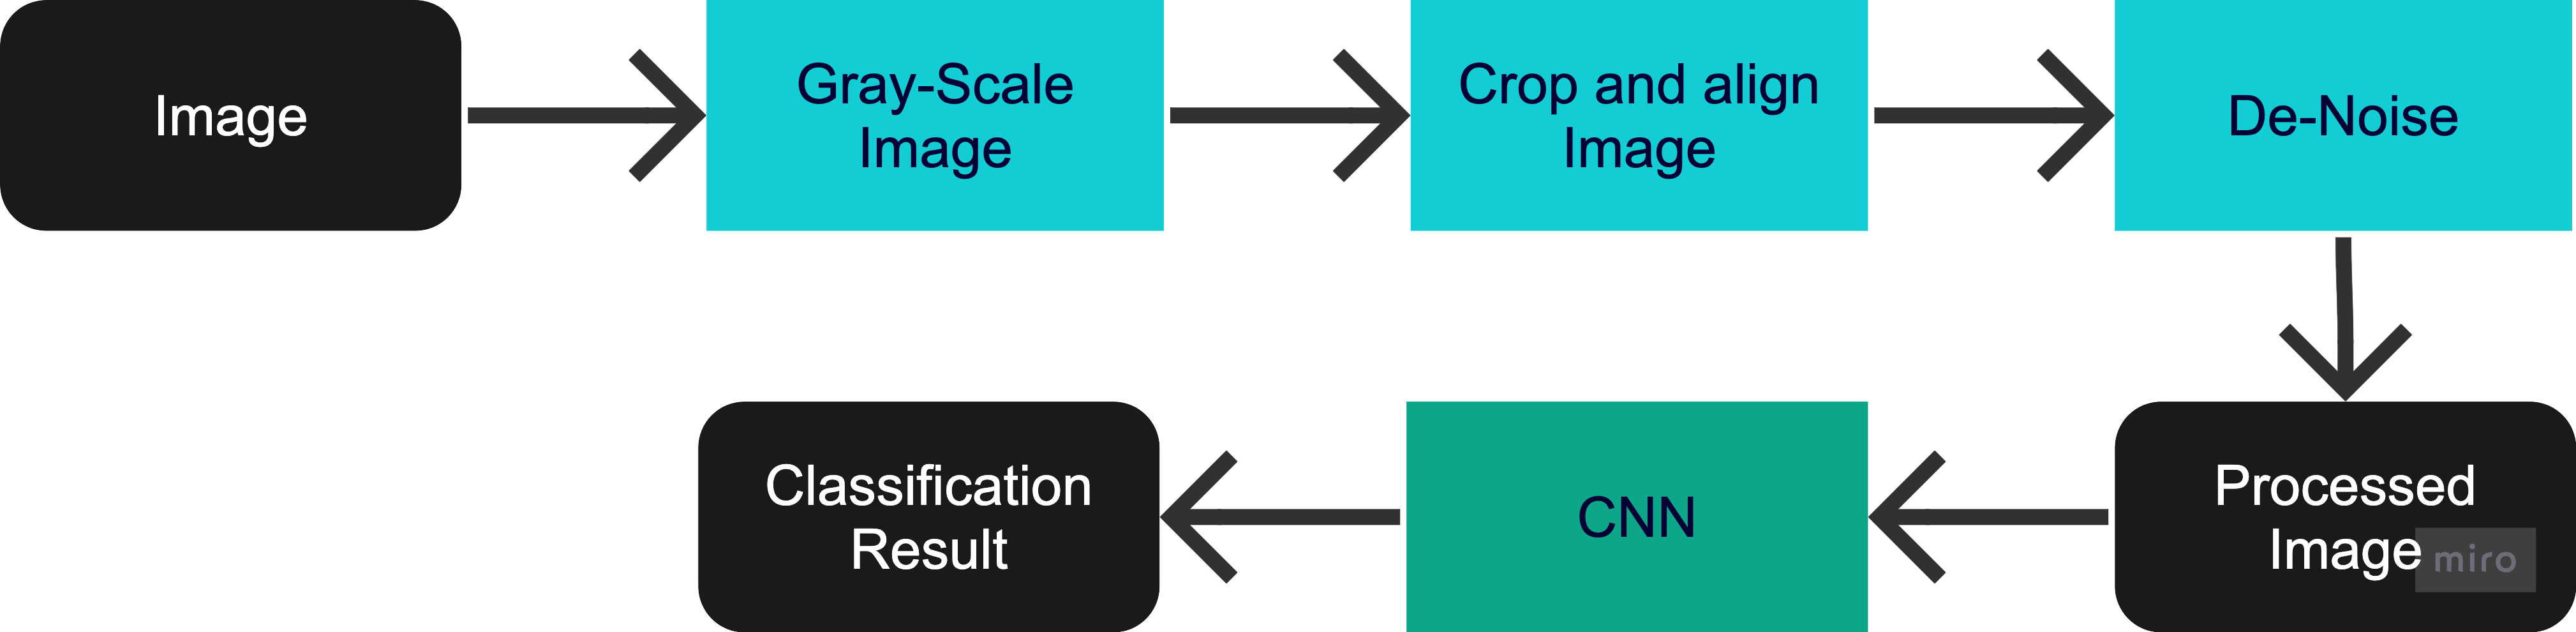
\includegraphics[width=0.9\textwidth]{images/fer-preprocessing-modelling.png}
\caption{Preprocessing and Modeling.}\label{fig:prep-mod}
\end{figure}

\newpage
\section{\acrlong{ser}}
To achieve Emotion Recognition through speech, we will follow two approaches: 
\begin{enumerate}
    \item using \emph{phonological} information (pitch, amplitude, spectral features, etc.)
    \item using \emph{semantic} information (words, grammar)
\end{enumerate}

\vspace{5mm}
% Jana's task:
%\emph{1. Approach: phonological information}

\noindent For the first approach, we will create a \acrfull{crnn},  i.e. a sequential neural network with 1D convolutional layers. It will take the spectrograms as input that we obtained through preprocessing and outputs the most likely emotion associated with the input. Here, the python library Keras can be used to easily build a neural network by adding desired layers to the model. Keras is open-source and available for free. \\

%\noindent \emph{2. Approach: semantic information}
\noindent For the second approach, a combination of two neural networks will be used. First, an \acrfull{asr} model transforms the spectrograms into a textual representation of the utterance. This can again be done with Keras as it additionally offers APIs to pre-trained ASR models like DeepSpeech, an open-source model by Mozilla.
Then, the obtained text is assigned to an emotion by a transformer-based neural network. Here, the python library Hugging Face can be used. It is free, open-source and offers pre-trained transformer models like BERT. 
Since the ASR model and the transformer model are already pre-trained on a large corpus of data and our application scenario is kept general instead of domain-specific, it is not strictly necessary to find additional datasets for training the ASR model and the transformer model ourselves. \\

\begin{figure}[h!]
\centering
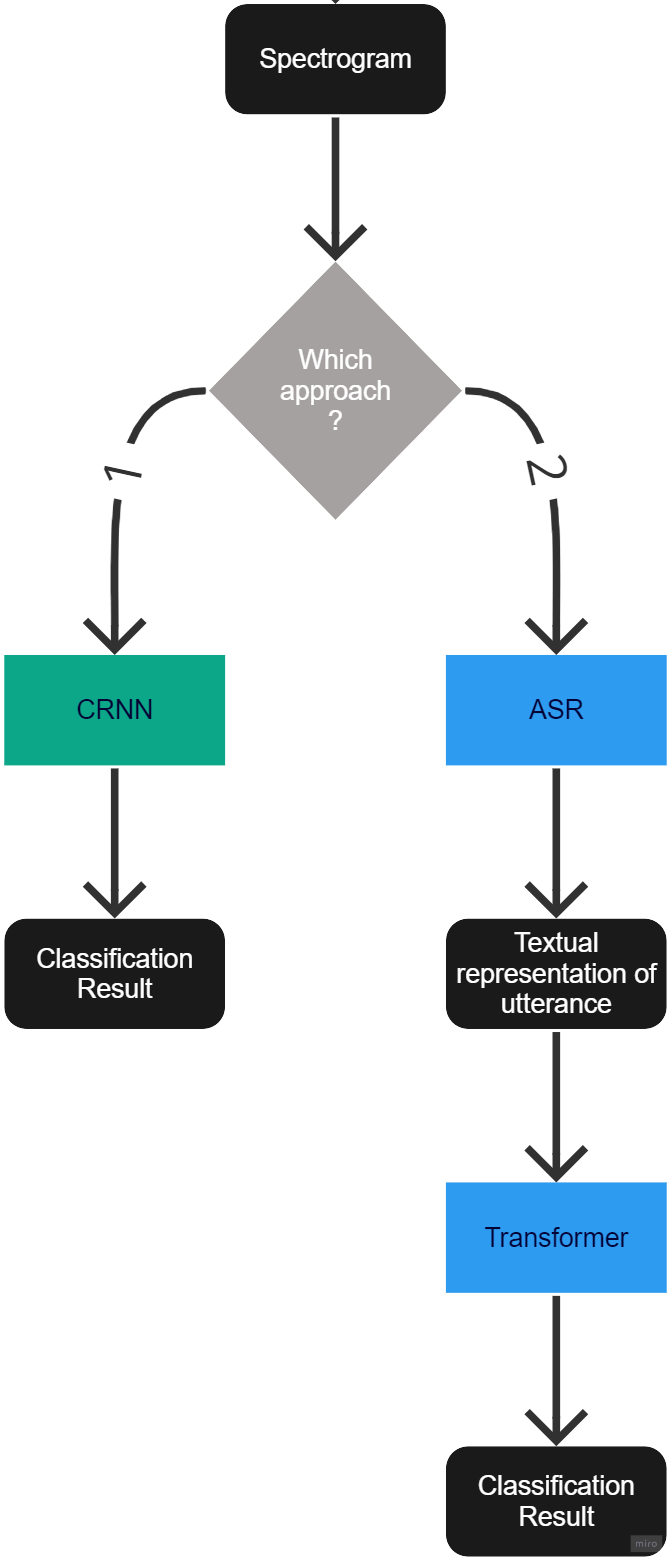
\includegraphics[scale=0.6]{images/SER_Modeling.png}\\
\caption{\acrshort{ser} Modeling.}\label{fig:ser_modeling}
\end{figure}

%\newpage
\section{Combined Emotion Recognition}
Finally, we aim to develop a combined system for facial and speech emotion recognition, as depicted in Figure \ref{fig:whole-system}. To do this we will first develop the separate facial and speech emotion recognition models as seen above. Once we have trained these models, we will try to integrate them into a single system and will then evaluate the performance of the combined system using standard evaluation metrics like precision and recall. Apart from that, we will again give the users the opportunity to give feedback through the GUI. 
\begin{figure}[h]
\centering
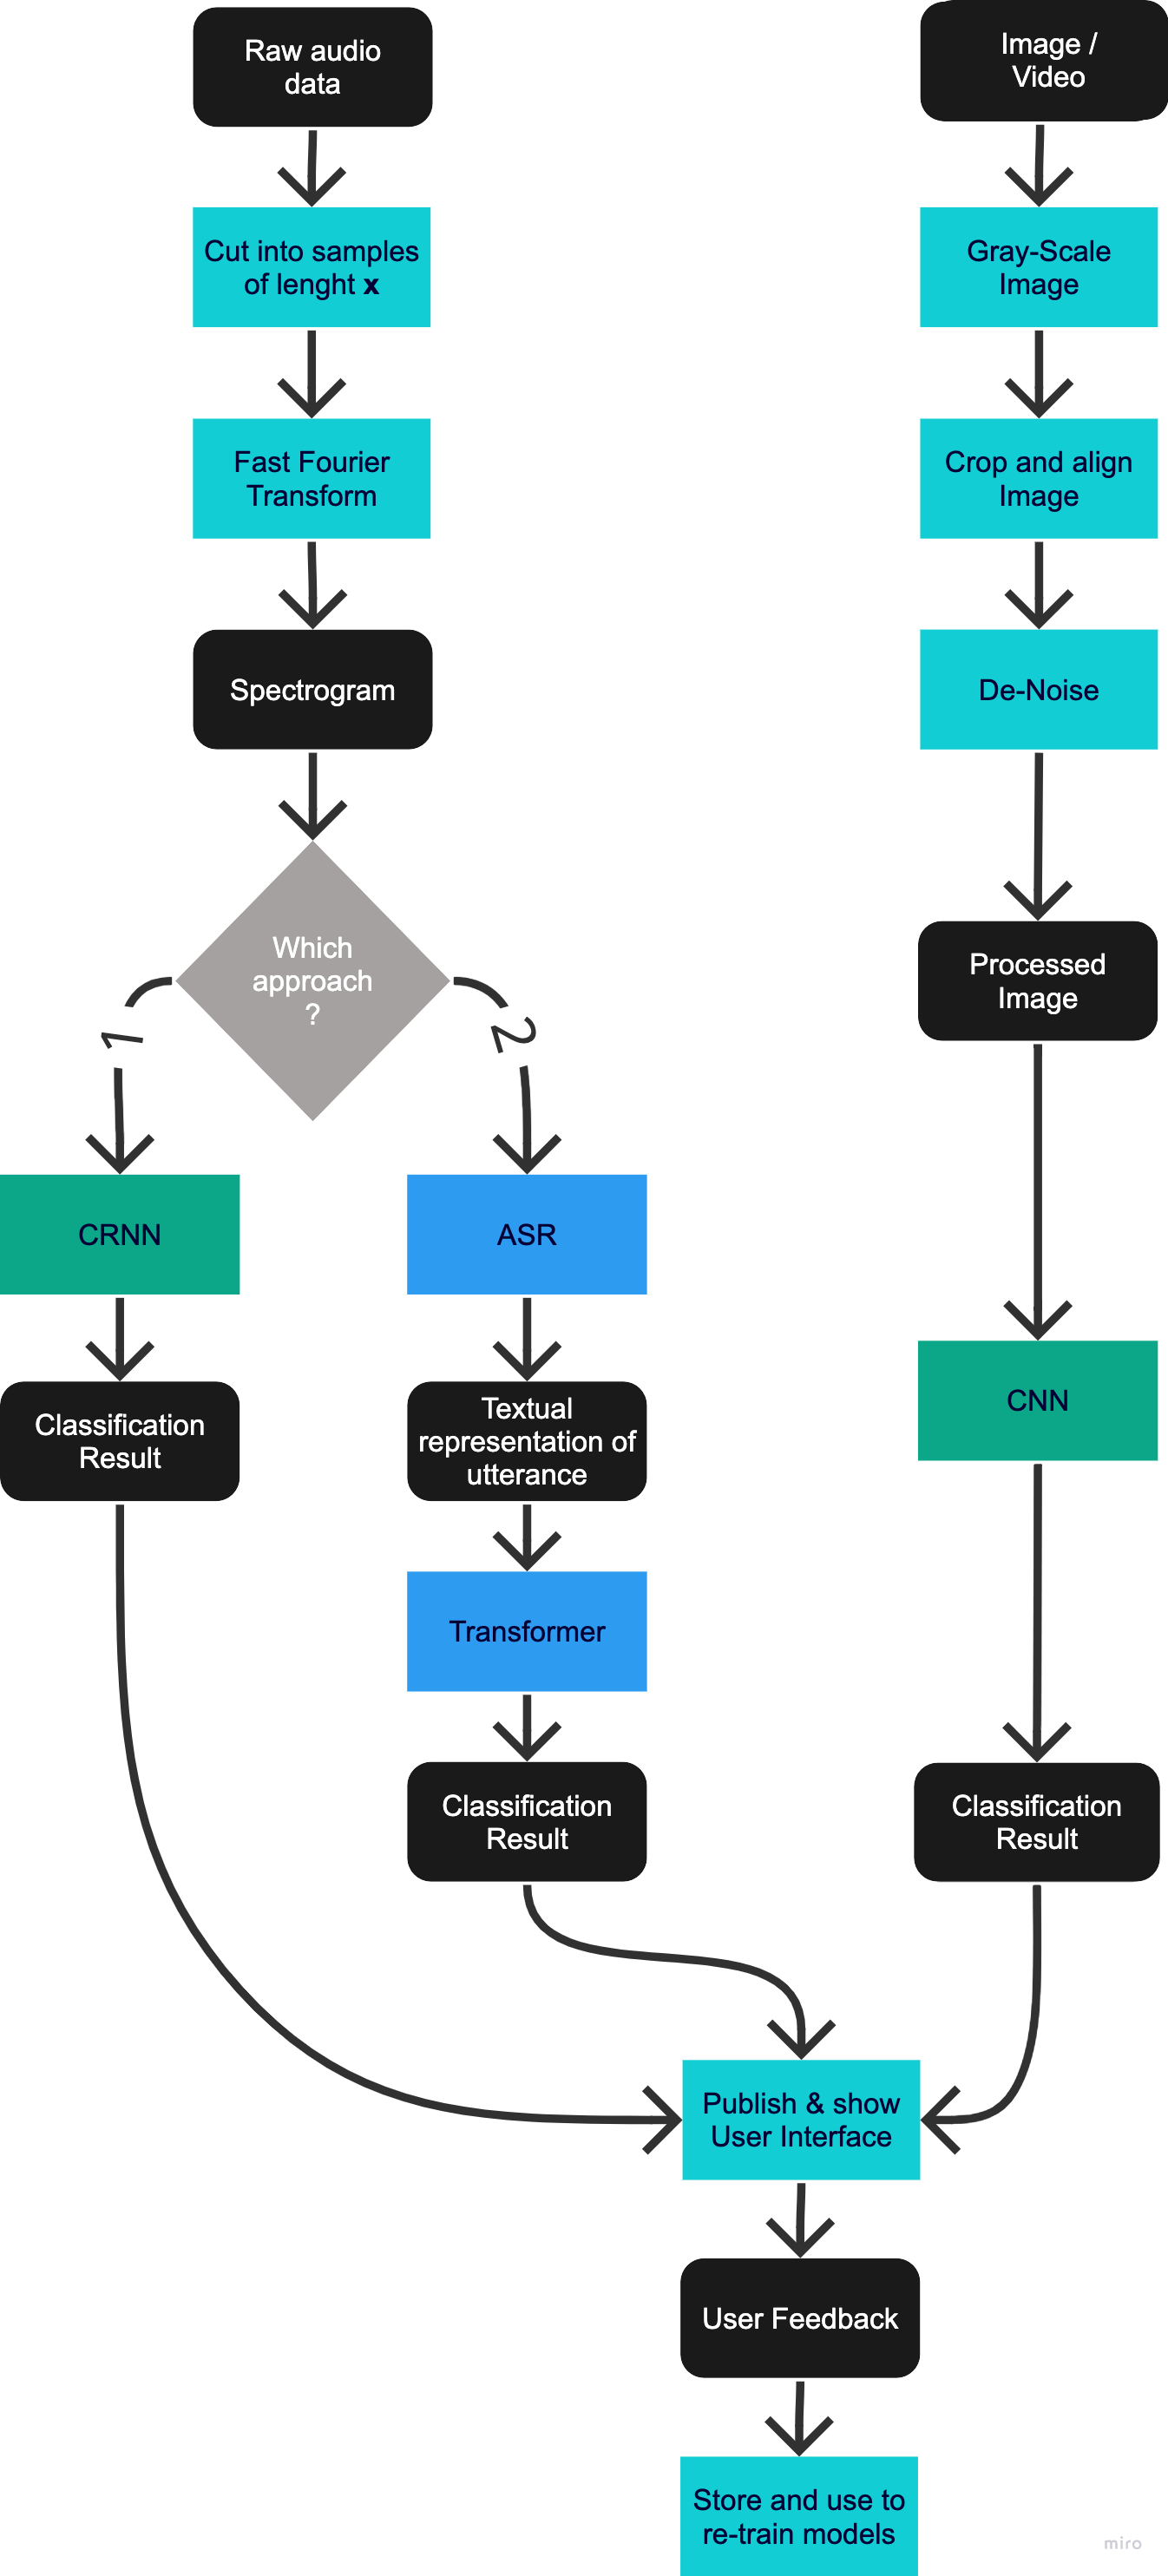
\includegraphics[width=0.7\textwidth]{images/whole-system.png}
\caption{Structure of the entire system}\label{fig:whole-system}
\end{figure}

\chapter{Model Evaluation}\label{chap:Evaluation}
%\input{texts/face/3_eval-fer}
%\input{texts/speech/3_eval-ser}
After training a model, the next goal is to test the model on new data. For this we can first use the test data and measure the accuracy, precision, recall and F1-Score. The goal is to keep a track of the precision and loss of the model in training. The model must have a loss under a certain value and a precision above a certain value. 

%TO-DO: put here a small paragraph about the use of cross validation that can be used and maybe formula of precision recall etc

During the development, we will also take advantage to unitary test for code coverage, these unitary tests will be needed to validate commit on the source control (GitHub in our case) of the project. Using this test will allow us to have an automated test pipeline that would be use for CI/CD. Additionally to the classic metrics for quality assurance, we allow the person captured by image and speech to input their actual emotion and comparing their actual emotion to the predicted one as will be described in the following section.


%Data splitting for Cross-Validation
%True positive (TP), True negatice (TN), False positive (FP), False negative (FN) when the model is not able to recognize any emotion.
%\begin{itemize}
%    \item Accuracy test,
%    By calculating how accurate is the model, using the following formula, $Accuracy = \frac{TP + TN}{N_{outputs}}$, we can test the success rate of the model.
%
%    \item Precision Test
%    Using the following formula, $Precision = \frac{TP}{TP + FP}$, we can test among the positive answers, the true positive rate.
%    
%    \item Sensitivity Test
%    $Sensitivity = \frac{TP}{TP + FN}$
%
%    \item Specificity Test
%    $Sensitivity = \frac{TN}{TN + FP}$

\chapter{System Deployment and Improvement}\label{chap:final-application}
To test both \acrshort{fer} and \acrshort{ser} in real-world scenarios, the trained models will be embedded in a pipeline to allow us to apply the trained model on real-world captured images and speech recordings. For \acrshort{fer} this can then in turn be applied to frames of a video, that will be captured by a camera, evaluating the emotions of one person (possibly multiple people if feasible). Accordingly, for \acrshort{ser} the users' utterances will be recorded with a microphone. Hereby, the continuous audio stream should then be cut every $x$ seconds to obtain the data samples. As Figure \ref{fig:whole-system} shows, both inputs will be preprocessed and fed into the respective models. The results from both of the approaches will then be continuously published on the user interface. Here, the users indicate whether one or both of the classifications are correct by stating their actual emotion through a small GUI. The user feedback will be stored along the respective image and audio sample and can then be used to retrain the model with more data, if the accuracy drops below a predetermined threshold. Overall, we aim to develop a robust and accurate combined system for facial and speech emotion recognition that can be applied to a range of real-world applications.

\begin{figure}[h]
\centering
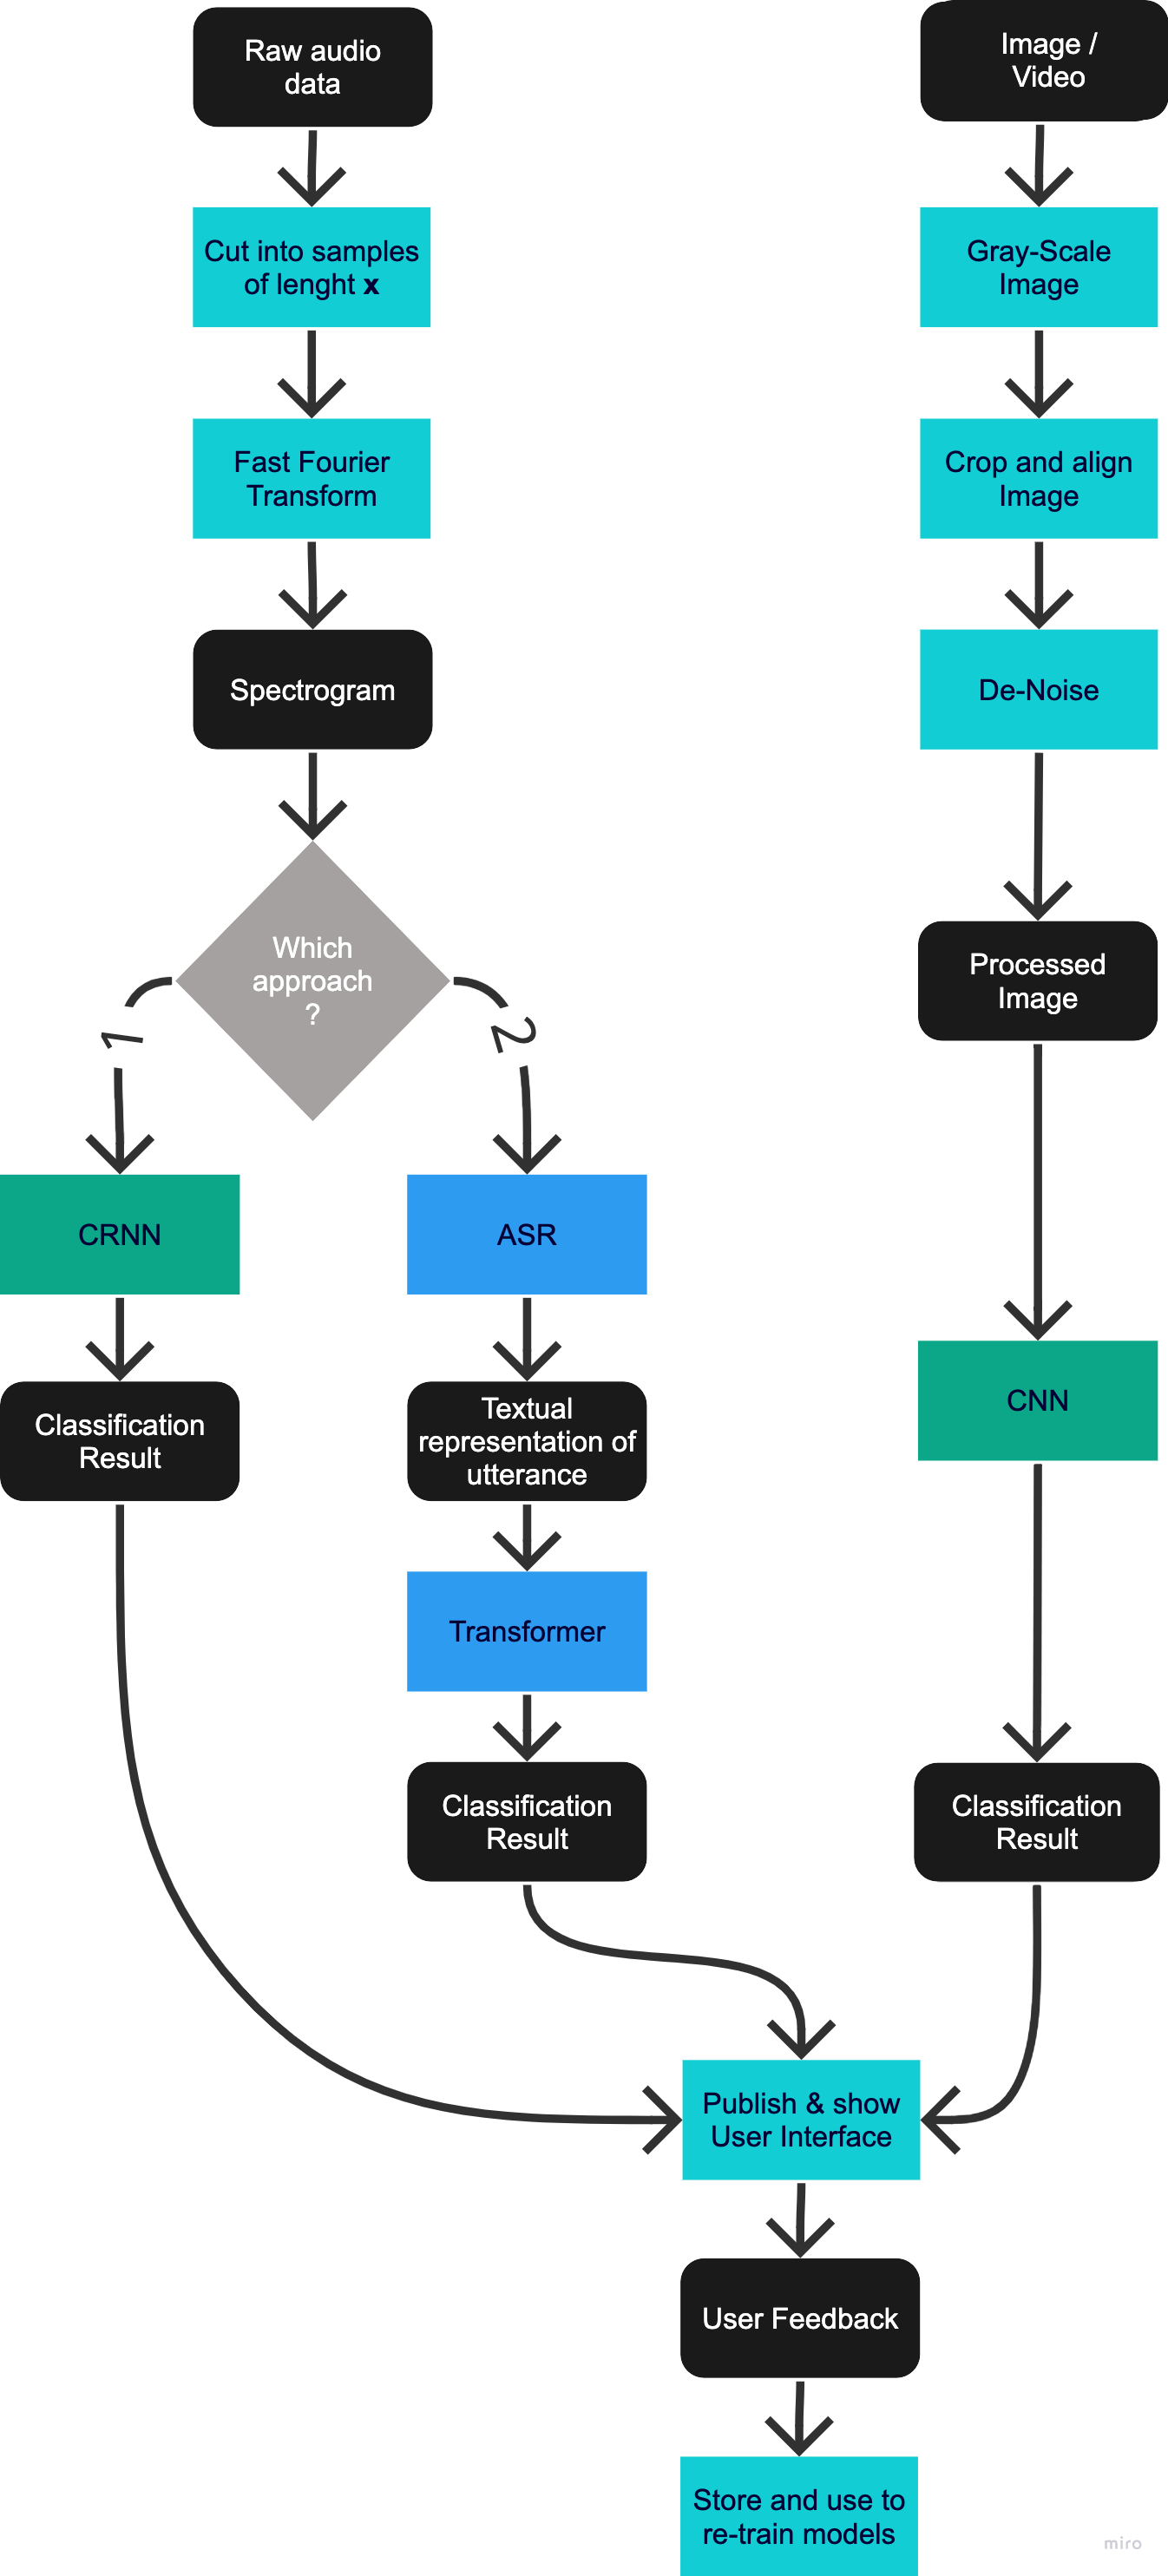
\includegraphics[width=0.7\textwidth]{images/whole-system.png}
\caption{Structure of the entire system}\label{fig:whole-system}
\end{figure}


%\chapter{Conclusion}\label{chap:conclusion}
%\input{texts/8_conclusion}
\cleardoublepage
\pagenumbering{Roman}
\setcounter{page}{\thesavepage}
\printbibliography[heading=bibintoc,title={References}]
\clearpage
%\clearpage
\end{document}
